\documentclass{ucasthesis}% thesis template of the Uni of Chinese Academy of Sciences
%% Multiple Options:
%% [scheme = plain] % for thesis writing of international students
%% [doublesided] % change to double-sided style, default is single-sided
%% [printcopy] % if printed, need this for a uniform binding width
%% [draftversion] % show draft version information, default is no show
%% [fontset = adobe] % use Adobe font
%% [standard options for ctex class]
%%%%% --------------------------------------------------------------------------------
%%
%%%%**************************Command Define and Settings*****************************
%%
\usepackage{commons}% common settings
%% usage: \usepackage[option1,option2,...,optionN]{commons}
%% Multiple Options:
%% [numbered] % default citation style. textual: Jones [1]; parenthetical: [1]
%% [authoryear] % author year citation style. textual: Jones (1995); parenthetical: (Jones, 1995)
%% [alpha] % alpha citation style. textual: not available; parenthetical: [Jon95]
%% [myhdr] % one available header and footer style, will enable fancyhdr
%% [lscape] % provide landscape layout environment
%% [geometry] % configure page layout by geometry package
%% [list] % enable enhanced list environments, useful for Algorithm and Coding
%% [color] % enable color package to use color, current package is xcolor
%% [background] % enable page background, will auto enable color package
%% [tikz] % enable tikz for complex diagrams, will auto enbale color package
%% [table] % enable a table package for complex tables, current is ctable
\usepackage{custom}
\usepackage{fullpage}

\begin{document}

\frontmatter

%%%
%%% >>> Title Page
%%
%%
%%% Chinese Title Page
%%
  \confidential{}% show confidential tag
  \schoollogo{scale=0.45}{Img/UCAS}% university logo
  \title[兰州大学本科毕业设计实践~\LaTeX{}~模板]{全局和局部特征提取算法在人脸图像领域的比较}
  \author{栾英杰}% name of author
  \advisor{路永钢~教授}% names and titles of supervisors
  \advisorinstitute{兰州大学}% institute names of supervisors
  \degree{本科}% degree
  \degreetype{工学}% degree type
  \major{电子信息科学与工程}% major
  \institute{兰州大学}% institute of author
  %\chinesedate{2014~年~6~月}% only need for user customized date
%%
%%% English Title Page
%%

  \englishtitle{Facial Decomposition Methods Comparison \\ Between Global and Local Approaches }
  \englishauthor{Yingjie Luan}
  \englishadvisor{Professor Yonggang Lu}
  \englishdegree{Bachelor}
  \englishmajor{Engineering}
  \englishinstitute{School of Information Science and Technology,\\ Lanzhou University}
  %\englishdate{June, 2014}% only need for user customized date
%%
%%% Generate Chinese Title
%%
\maketitle
%%
%%% Generate English Title
%%
\makeenglishtitle
%%

%%
%%% >>> Abstract
%%

\includepdf{add1}

\begin{abstract}

本项目以人脸图片为主要内容,就不同降维算法的性能进行了比较,并尝试就实际人脸识别中的算法及参数选择问题给以一些建议.其主要内容有:

\paragraph{基于全局的特征提取算法} 本文首先实现了PCA, NMF, ICA等全局特征提取算法,这些算法有压缩率大,运行效率较高的优点,但也有着无法辨别背景,识别率存在上限的缺点.在对这些特征提取算法比较之后,作者发现比较难以实现精确的人脸识别,于是便开始了基于局部的特征提取算法的探究.
\paragraph{基于局部的特征提取算法} 本文以SIFT算子为例,实现了局部的特征提取算法.并对SIFT算子进行了一定的优化.SIFT相比较PCA算子,具有能区分背景,基于图像变换最大,信息最多的地方描述的优点.但是,也同时发现了SIFT算法计算速度较慢,内存占用大的缺点.
\paragraph{模型分析} 在实现上述内容的过程中,不可避免的出现了构建降维,分类等模型,并就模型的优劣进行比较.本项目也就机器学习中基本的模型比较过程进行了实践.



\keywords{本科课程实践,特征脸, 局部特征提取算法, 分类算法}
\end{abstract}


\begin{englishabstract}

The initial purpose of this project is to test the performance of different \textbf{Decomposition Algorithms} in terms of \textit{Facial Images}. PCA, NMF, ICA were implemented and has successfully compressed facial images with around 10,000 pixels into vectors of length 30 to 100. Besides that, a simple face recognition system was built with SVM as the classifier and the overall accuracy of successful recognition can be around 85\%. \newline

\textbf{Component-based approaches} were presented to conquer problems brought by the \textbf{global approach}. In comparison to global 
approaches, it only concentrates on the areas of images with the largest changes(or with maximum energy). And can provide a more accurate description of people. SIFT were implemented, and the overall accuracy can be 99\% at its maximum. \newline

Besides \textbf{global approach} and \textbf{component-based approaches}, this project also implemented  common frameworks for model evaluation. Both for the decomposition algorithms and classification algorithms.


\englishkeywords{Eigenfaces, Classification Algorithms, Component-based Feature Extraction, SIFT, Model Evaluation}
\end{englishabstract}
 %title etc..
\tableofcontents

\mainmatter
%%%%% --------------------------------------------------------------------------------
%%
%%%%********************************Main Content**************************************
%%
%%% ++++++++++++++++++++++++++++++++++++++++++++++++++++++++++++++++++++++++++++++++++
%\chapter{项目介绍}

\section{项目目标}

本项目在于尝试特征提取算法,具体来说,本项目以人脸图像为例,就人脸图像的特征提取展开了讨论.主要分为两个部分.
\paragraph{基于全局的特征提取算法} 本文首先实现了PCA, NMF, ICA等全局特征提取算法,这些算法有压缩率大,运行效率较高的优点,但也有着无法辨别背景,识别率存在上限的缺点.在对这些特征提取算法比较之后,作者发现比较难以实现精确的人脸识别,于是便开始了基于局部的特征提取算法的探究.
\paragraph{基于局部的特征提取算法} 本文以SIFT算子为例,实现了局部的特征提取算法.并对SIFT算子进行了一定的优化.SIFT相比较PCA算子,具有能区分背景,基于图像变换最大,信息最多的地方描述的优点.但是,也同时发现了SIFT算法计算速度较慢,内存占用大的缺点.\newline


本文从以上两个角度来对人脸图像的特征提取算法进行了分类,并尝试通过模型比较的方法来为实际应用中的算法,参数选择提供参考.

%\todo{Background Research}

\section{项目范围}
人脸识别是一个比较大的内容,它主要分为以下几个步骤:
\begin{enumerate}
	\item{基本的图像处理:} 这一部分把人脸图像做普通的图像处理,使用基本的图像处理算法,来进行如加深对比度,亮度平衡,去噪等操作.
	\item{人脸检测:} 由于很多情况下人脸并非实际应用图片中的唯一物体,大多数情况下需要使用算法在普通图片中识别出人脸来单独处理.
	\item{降维操作:}  由于人脸图像作为由灰度值或彩色值表示的矩阵,直接处理中存在着类内差别大,向量维数大,数据冗余度高等诸多缺点.需要将人脸图像的特征提取出来,并具体就其特征深入处理.
	\item{识别操作:} 提取出人脸的特征后,人脸识别问题就被转化为经典的机器学习问题了.可以把模型描述为"给定了人脸的特征向量,来恢复人脸标签"的监督或非监督机器学习问题.
\end{enumerate}

而本项目主要探究的话题在于问题3,也就是给定了人脸图像,从中提取更有表现力的特征向量的问题.从这个角度上,本文从多个角度,提取了多种特征向量,并结合了多种分类算法,来探究不同特征提取算法,及同一特征提取算法不同参数下的性能优劣.
\section{本项目报告的结构}
\begin{enumerate}
	\item 本报告第一章是关于项目的简单介绍
	\item 本报告第二章详细介绍了多种基于全局的特征提取算法
	\item 本报告第三章以SIFT算子为例,介绍了基于局部的特征提取算法
	\item 本报告第四章从多种角度(类间距离,结合分类机等)对前两章节实践的特征提取模型加以比较
\end{enumerate}
\section{用到的数据库}
本文用到了ORL数据库\cite{samaria1994parameterisation},ORL数据库由40人每人10张不同角度共计400张图片组成.

ORL数据库举例:
	
	\begin{center}
	\begin{minipage}[t]{\linewidth}
	%\label{fig:main}
	\center
	{
	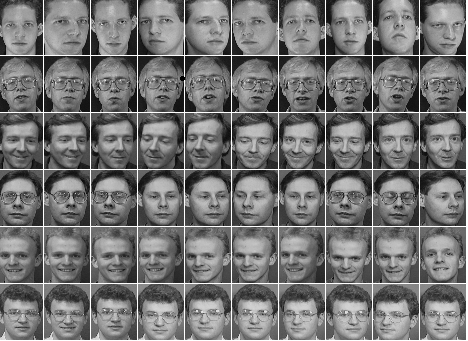
\includegraphics[width=\textwidth]{Img/faces} \captionof{figure}{ORL数据库举例}
	}
	\end{minipage}
	\medskip
	\end{center}
		
\section{项目应用}
值得一提的,本项目虽然是就人脸图片算法展开了讨论,但是实际应用并不仅限于此.在大多数处理过程中,人脸图片被展开并作为较长的向量处理,而之后对这个展开后向量的操作就可以被应用到其他高维数据的处理上去.本文中所讨论的算法可以有效的降维,减小数据冗余.\newline


其他可以应用高维处理算法的问题有:

\begin{itemize}
	\item{基因处理: } 基因是由A, T, C, G四种碱基组成序列,通常长度可以达到10-15k\cite{twine2011whole}.降维算法和特征提取算法可以更加有效地识别出基因的特征,从而帮助建立性状和基因的关系.
	\item{乐曲识别:} 乐曲可以被视作很长的电信号序列.在音乐幅值谱上的特征提取可以识别音乐的流派,歌手等信息.
\end{itemize}



\section{本项目内容及真实性声明}

本项目大部分代码都在\textit{Matlab 2015b}下运行,本报告由 \LaTeX 撰写. 同时项目及项目报告都使用了\textit{Git}来进行项目管理.主要内容有:
\begin{enumerate}
	\item \url{https://github.com/y1275963/Eigenfaces} 项目的主体内容,包括了基本代码的实现
	\item \url{https://github.com/y1275963/bachelor_thesis} 项目报告的主体内容,包括文章本身及文章中的插图
	\item \url{https://www.dropbox.com/sh/zlie193xdxog7i7/AACAmN5ddQE0-Fn9NgGLeSIsa?dl=0} 本地运行结果缓存, 由于很多情况下,本项目涉及了参数扫描的过程,这些过程运行时间比较长,因此为了方便绘图的缘故也对结果进行了缓存
\end{enumerate}

在项目报告的附录中,详细罗列了使用到的软件库及原始数据,同时也简略罗列了开发记录.\newline


作者在此声明,文章中所有出现的图片,表格均由作者本人亲自得到,并在项目报告中尽力详细描述了具体实现中的参数选择.

\section{主要算法实践情况}
\begin{itemize}
	\item \textbf{PCA}: 自己实践
	\item \textbf{NMF}: 自己实践
	\item \textbf{ICA}: \textit{FastICA for Matlab 7.x and 6.x, Version 2.5}
	\item \textbf{SIFT}: \textit{VLFeat, Version 0.9.20}
	\item \textbf{NKNN}: 自己实践
	\item \textbf{SIFT-PCA}: 自己实践
	\item \textbf{SVM}: \textit{LIBSVM, Version 3.21}
	\item \textbf{分类机遍历}: \textit{Matlab2016a APP: Classification Learner}
\end{itemize}
%\chapter{基于全局的特征提取算法}
\label{cha:global}
\section{基本框架}
PCA\cite{turk1991face}是近代人脸识别中较早的方法.在文献中,作者于1991年评价了之前基于人脸手工的标定,专家模型构建的方法,并且指出了人工方法的若干不足之处.同时提出了基于统计的PCA方法,成功实现了自动的人脸识别系统.并且,作者提出了\textit{eigenface}这个用来表征人脸图像投影的空间.从那以后,研究者们从多个角度研究了许多除了\textit{eigenface}以外的方法,提出了\textit{fisherface}\cite{kwak2005face}等一系列特征空间.

这些基于统计的方法都有着不同的出发点,但在实现上都是比较相似的.他们从不同的角度来尝试从人脸数据库中分解出更有代表性的分量,并把那些分量作为特征空间的基底.当处理新入样本时,新的样本和创建的特征空间基底作投影操作,得到的样本坐标就是该样本在空间的表示.以下是本文中所尝试的方法及其主要思想:
\begin{center}
  \footnotesize
        \captionof{table}{本文中所尝试的降维方法及其主要思想}
  \begin{tabular}{l|c}
  \hline 
    方法 & 主要思想 \\ \hline
    PCA & 在假设样本高斯分布的情况下,寻找样本空间特征值最大的k个正交向量作为基底\\ \hline
    NMF & 由于图片仅由正实数表示,提出了保证特征向量也为正数的前提下的特征分解方法\\ \hline
    ICA & 在假设样本独立统计(I.I.D)及非高斯分布的情况下,来近似估计各个独立分量成分\\
    \hline
  \end{tabular}
\end{center}
\subsection{人脸分解的例子}
下面以PCA为例,来表示一个具体的基于全局的人脸特征提取算法的工作流程.
\paragraph{构建基底空间} 这一步骤是不同方法的主要区分之处,不同的算法主要是从不同的角度来构建更为优化的投影空间,使得投影后的样本坐标更具有表现力.
\newline
下面是通过分解ORL数据库所有图片得到的前6张特征脸(\textit{eigenfaces})和平均脸:

\begin{center}
\begin{minipage}[t]{\linewidth}
%\label{fig:main}
\center
{
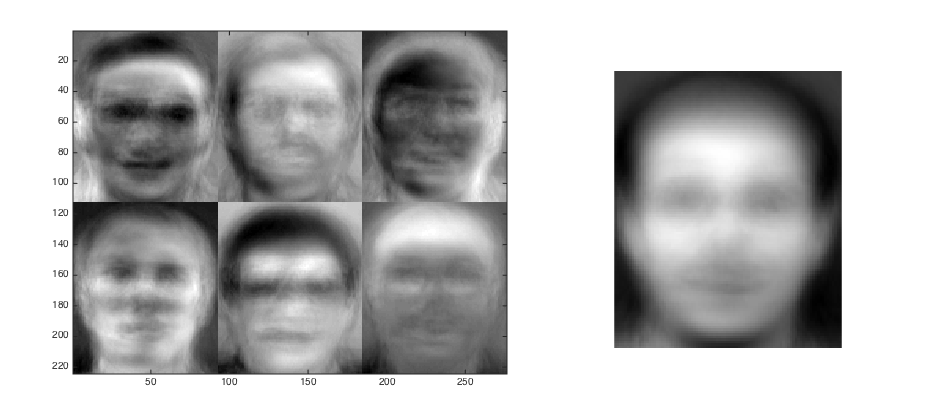
\includegraphics[width=\MyFactor\textwidth]{Img/pca_eigenspace.png} \captionof{figure}{前6张特征脸和平均脸}
}
\end{minipage}
\medskip
\end{center}

其中,PCA的计算在给出特征向量的同时,还会给出代表特征向量权重的特征值,上述6个特征值在400个特征向量空间中占据了51.4\%的权重.权重分布如下图:

\begin{figure}[!htbp]
\centering 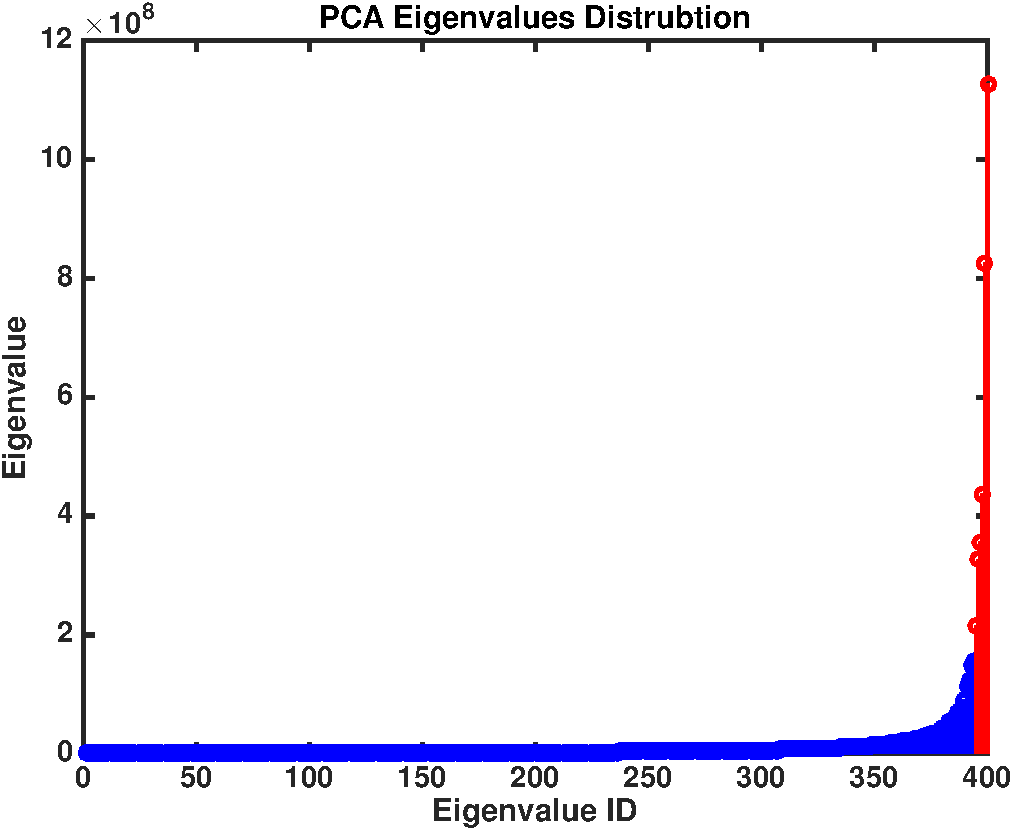
\includegraphics[width=\MyFactor\textwidth]{Img/pca_eivalue.pdf} 
\caption{特征值分布图 \\ 蓝色:舍弃的特征向量, 红色: 保留的特征向量}
\end{figure}
设特征向量组成的基底矩阵为V, 输入图像为I, 则该步骤可以表示为:
\begin{equation}
Weights = Inv(V) \cdot I
\end{equation}
其中
\begin{itemize}
	\item V为一个$m  \times  n$的矩阵,m是特征脸的像素数,n是特征向量的数目,$Inv(V)$为其转置矩阵
	\item I为一个$m \times d$的矩阵,m是特征脸的像素数,d是需要分解的输入图像数目
	\item Weights为一个$n \times d$的矩阵,n是特征向量的数目,d是需要分解的输入图像
\end{itemize}


本例中图像在特征向量空间下的权值如下:
\begin{center}\begin{tabular}{|l|l|l|l|l|l|}
\hline
-123.7915&-689.9194&261.7842&1867.0258&1072.1813&1531.176\\\hline
\end{tabular}
\end{center}

\paragraph{输入样本重构} 这一步是根据上一步求得的权值来线性地重构这张输入样本.当然了,当实际应用时不需要恢复原始输入图片时,这一步可以省略.

\begin{center}
\begin{minipage}[t]{\linewidth}
%\label{fig:main}
\center
{
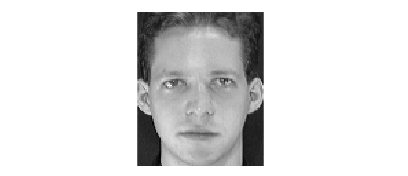
\includegraphics[width=\MyFactor\textwidth]{Img/pca_sample.png} \captionof{figure}{左:输入图像 右:重建后的图像}
}
\end{minipage}
\medskip
\end{center}

	
	以下是该流程的简要示意:
\begin{center}
\begin{minipage}[t]{\linewidth}
%\label{fig:main}
\center
{
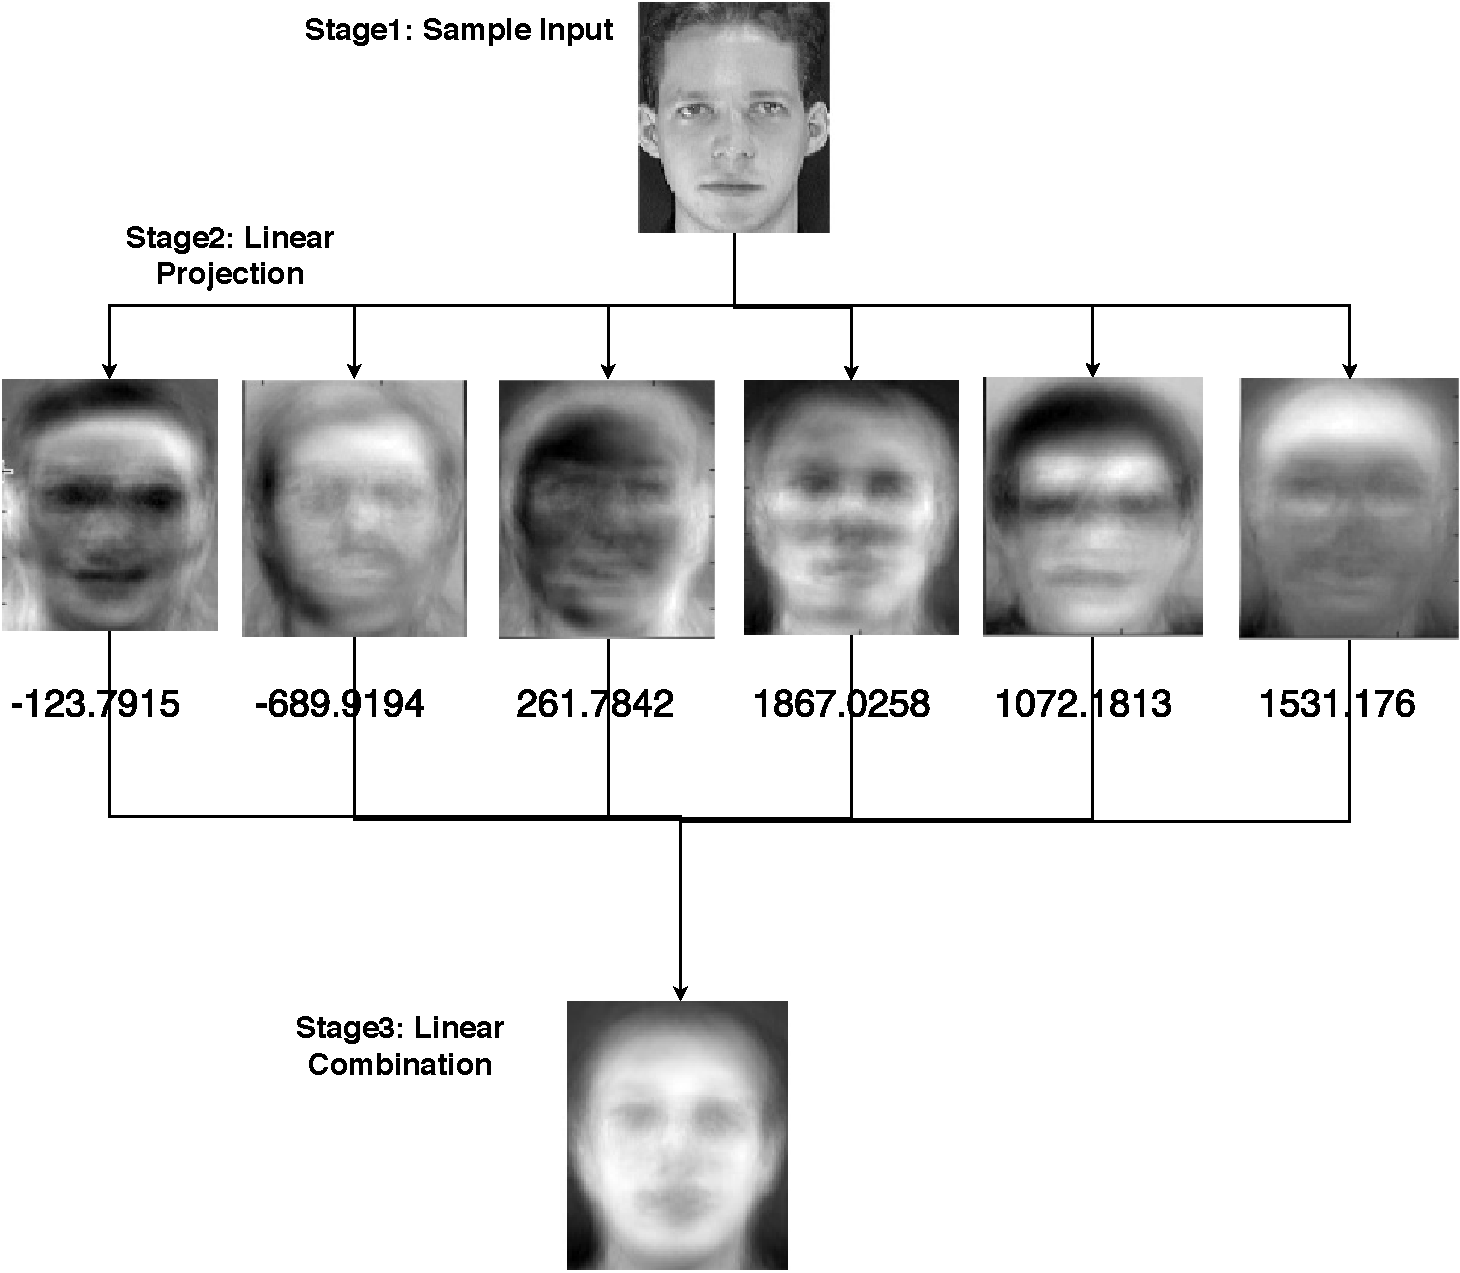
\includegraphics[width=\MyFactor\textwidth]{Img/pca_demo.pdf} 
\captionof{figure}{图像投影示意}
}
\end{minipage}
\medskip
\end{center}

\subsection{两类不同的特征空间}
\label{sec:arch2}
\begin{center}
\begin{minipage}[t]{\linewidth}
%\label{fig:main}
\center
{
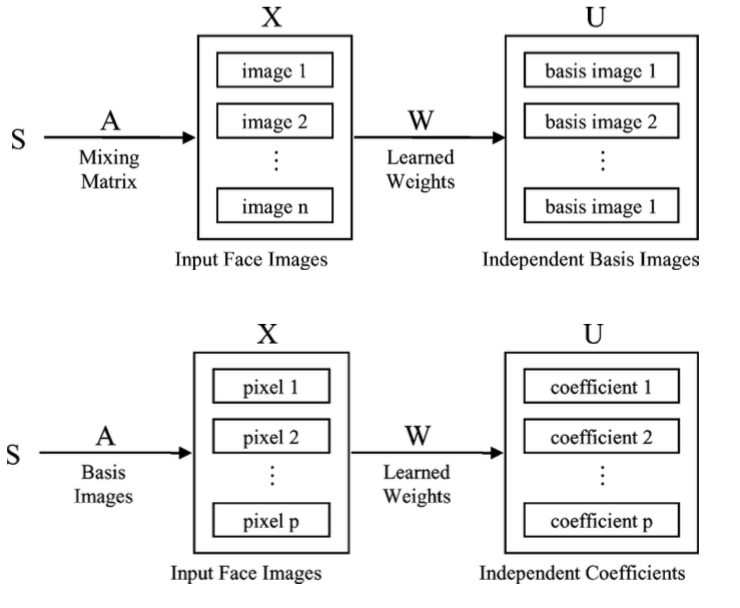
\includegraphics[scale=1]{Img/ica_c1c2.png} 
\captionof{figure}{图像投影示意 \\ 上: Architecture I, 下: Architecture II. 来源\cite{draper2003recognizing}}
}
\end{minipage}
\medskip
\end{center}
值得指出的是,受到\cite{draper2003recognizing}启发.这里同时存在着两类不同的分解思想.他们的区别在于一类的输入样本是另一类的转置.\\



第一类的思想是将人脸图像作为变量而将每张图像上的像素作为这个变量的描述,而分解的操作发生在人脸的空间上.


第二类的思想是将人脸图像样本作为各个像素的描述,并且转而把像素作为变量.
\\
在实践中由于第二类的维数过高,运算量太大,采用了第一类.

\section{PCA}
本章节的主要依据文献是\cite{turk1991eigenfaces, turk1991face},从本章节开始,将依次简要介绍PCA, NMF, ICA的基本原理和计算方法.并在ORL数据库下给出其特征脸空间. \newline

根据\cite{de2010face, smith2002tutorial},当PCA的运算数据中减去其平均值(又称为平均脸),PCA运算等价于KL运算.所以本文也是对KL运算的介绍.\newline

\subsection{PCA的思想}
\begin{enumerate}
	\item 记$\tau_i$为由第i张基底计算集图像形成的图像.原始图像是一个$m \times n$大小的矩阵,$\tau$为一个原始图像按照行展开形成的$ m \times n$长的行向量
	\item 记\begin{equation}\Phi = \frac{1}{M}\Sigma_{n-1}^M\tau_n\end{equation}$\Phi$是$\tau_i$的平均值,也就是这个基底计算集的平均脸,M是基底计算集的样本数目
	\item 记\begin{equation} \label{Centering} \phi_i = \tau_i - \Phi\end{equation}
	\item PCA旨在选择值最大的若干$\lambda$,\begin{equation} \lambda_k = \frac{1}{M}\Sigma^M_{n=1}(u^T_k \phi_i)^2\end{equation} 同时,$u_k$受到正交性的限制:\begin{equation}\label{pca:corr} u_k \times u_l = \left\{\begin{array}{c}
        1(k = l)\\
        0(k \neq l)
    \end{array}\right.
    \end{equation}其中$\lambda$被称作特征值,$u$被称作特征向量,也就是所求的特征基底.
	\item $\lambda_k$的个数是需要选择的,选择的特征向量数越多,保留的内容就越多,但同时压缩效果就越差
\end{enumerate}
\subsection{PCA的计算方法}
从线性代数的角度,PCA相当于最小化这个样本集的二阶统计值,当PCA完成后,各个特征向量之间的相关性为0.而$u$,$\lambda$分别为相关矩阵C的特征值,特征向量.
\begin{equation}
	C = A \cdot A^T
\end{equation}
A是样本集,也就是$[\phi_1, \phi_2,...,\phi_M]$\\ 

由于C为一个$(m \times n) \times (m \times n)$大小的矩阵,直接计算不便,经分析,对C的计算等价于对L的计算,L定义为
\begin{equation}
	L = A^T \cdot A
\end{equation}
L是一个$M \times M$大小的矩阵.
而计算过程也就是计算L矩阵的特征向量,特征值.而此时的特征向量$v$并非直接可用的向量,其大小为$M \times M$,而选择过k个特征值最大的的向量后,其大小为$M \times k$,需要使用计算
	\begin{equation}
		u=A \cdot v
	\end{equation} 
	便得到了大小为$(m \times n) \times k$的特征基底.
	
\subsection{PCA的在ORL测试集的投影基底}
以下是使用ORL数据集400张图片作为基底,选择特征值最大的前64张图片得到的特征基底.
\begin{center}
\begin{minipage}[t]{\linewidth}
%\label{fig:main}
\center
{
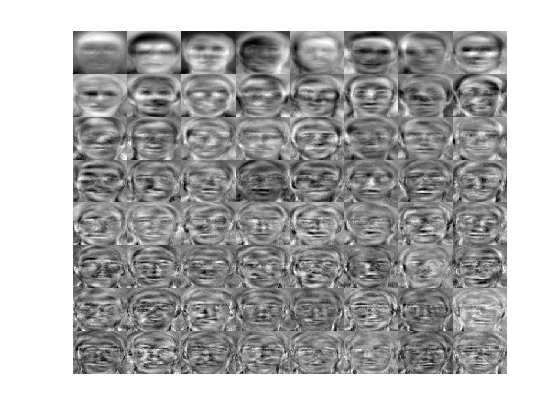
\includegraphics[width=\textwidth]{Img/pca_base.png} \captionof{figure}{PCA的在ORL测试集的投影基底}
}
\end{minipage}
\medskip
\end{center}

同时需要注意的是,PCA所得到的基底是特征向量,而特征向量之间由\ref{pca:corr}满足正交性,所以特征向量$Basis = [u_1,u_2,...,u_k]$构成的矩阵是正交矩阵,满足$Basis' = Basis^T$. 为了说明这一点,以下是上述基底两两之间的相关距离根据\ref{pca:corr}计算得到的距离矩阵:
\begin{center}
\begin{minipage}[t]{\linewidth}
%\label{fig:main}
\center
{
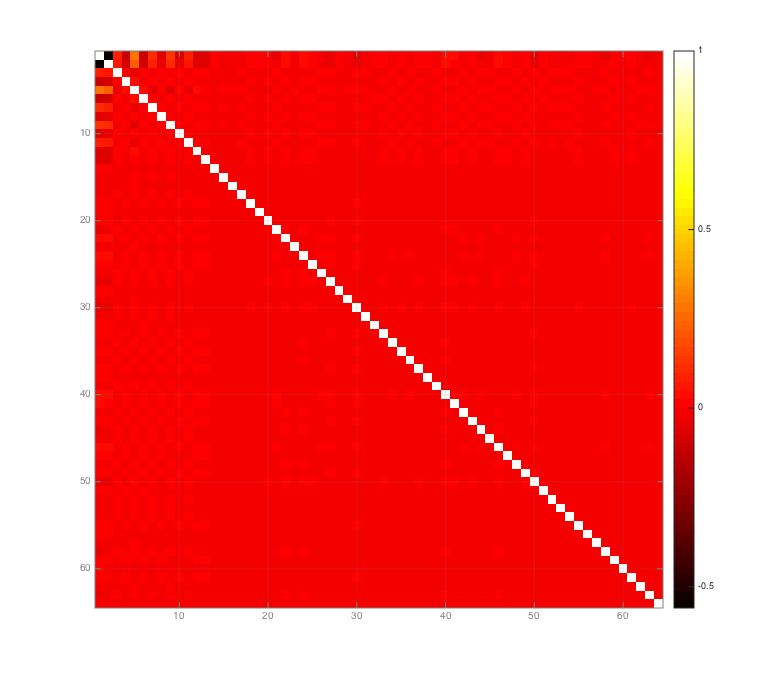
\includegraphics[width=\MyFactor\textwidth]{Img/pca_correlation.png} \captionof{figure}{PCA基底的正交性}
}
\end{minipage}
\medskip
\end{center}
由上图可见,大部分基底之间的相关性均接近于0.

\section{NMF}

\subsection{NMF的思想和计算方法}
本章节的内容主要基于\cite{lee1999learning, lee2001algorithms}.\newline

NMF算法围绕着在保证分量非负性的同时达到$V=W \cdot H$的分解.
	其中
	\begin{enumerate}
		\item V与等价于上一章节的$[\tau_1, \tau_2,...\tau_M]$,是基底计算样本的全集.
		\item W为一个$(m \times n) \times k$的矩阵
		\item H为一个$k \times m$的矩阵.可以由此得到$W \cdot H$是一个$(m \times n) \times M$的矩阵,和V有相同的形状.
	\end{enumerate}
 NMF定义了惩罚函数\begin{equation}
 \label{nmf_cost} ||V-W\cdot H|| = \Sigma_{ij} = (V_{ij} - WH_{ij})^2\end{equation}来描述分解的效果.$||V-W\cdot H||$是V和WH之间的欧式距离.实现完全分解时$||V-W\cdot H||=0$

NMF算法提出了保证W,H非负性的前提下的迭代公式,并证明了其收敛性,使用迭代的方法来逐步逼近最终的W,H.其迭代公式如下
	\begin{equation}
		\label{equ: nmf_iter1}
		H_{au} = H_{au}\frac{(W^TV)_{au}}{(W^TWH)_{au}}
	\end{equation}
	\begin{equation}
		\label{equ: nmf_iter2}
		W_{ia} = W_{ia}\frac{(VH^T)_{ia}}{(WHH^T)_{ia}}	
	\end{equation}
可以看到H,W的迭代运算中使用的仅仅是除法,乘法和加法,而同时V矩阵初值均为正数这就保证了H,W的非负性.

完成迭代后,舍弃H,认为W矩阵就是这个数据集的非负分解结果,也就是这个数据集的特征向量基底.\newline

同时,需要注意的是
\begin{itemize}
	\item 上述的迭代公式并非全局最优解.对于$||V-W\cdot H||$这个优化函数,目前并没有可以同时优化W和H的方法.NMF方法采用的是迭代的方法,也就是,优化H时,以上一步的W为目前最佳W,优化W时,以上一步的H为目前最佳H.而其该局限性使得这种优化方法只能收敛到局部最小值,并且每次结果都和初始值有关.\cite{berry2007algorithms}.
	\item 上述的迭代公式,惩罚函数只是NMF思想的一种实现方式.现实中还有其他的替代方法.在\cite{lee1999learning, lee2001algorithms}就列写了另一个惩罚函数和对应的迭代公式,还有对应迭代公式收敛性的证明.其惩罚函数为$$\Sigma_{ij}A_{ij} log \frac{A_{ij}}{B_{ij}} - A_{ij} + B_{ij}$$
\end{itemize}

\subsection{NMF的终止条件}
在\cite{lee1999learning, lee2001algorithms}中,并没有对NMF算法的终止条件作出说明,而NMF算法的终止条件也有很多种不同的解释,由于实际计算中很难达到理想的$V=WH$的条件,因此需要在算法收敛速度较慢时提前终止算法.
\begin{itemize}
	\item 在\cite{hoyer2004non}的算法中,其NMF算法是一个无限循环,而需要用户根据W和H的分解情况来自行中断程序.
	\item 在\cite{brunet2004metagenes}中,其NMF算法根据分析结果是否不再变化达到稳定而中断程序.
\end{itemize} 

本文的方法采用和\cite{brunet2004metagenes}类似的方法,这是一种经验方法,矩阵C的构建仅仅是为了描述结果的结构.具体来说,它的工作方法是:
	\begin{enumerate}
		\item 首先对于H矩阵(其形状为$k \times m$),得到每栏k个元素中最大值的位置,其取值从1到k,共计有m个
		\item 对这m个元素构成的向量Vect,构建对称布尔矩阵C,其中$C_{ij}$和$C_{ji}$为真代表Vect向量中第i个元素的位置和第j个元素的值相同.这在H矩阵中,代表的含义是第i列列向量中最大值的位置和第j列列向量中最大值的位置一样
		\item 迭代时,比较C和之前结果,如果差别比较小(本项目中为小于15个元素的差别),则认为迭代已经进入了稳定
		\item 当连续若干次C都和上一次迭代有近似相同结果时(本项目中设定连续6次),则终止程序
	\end{enumerate}

以下是使用该方法后某次的运行结果,
\begin{enumerate}
	\item 第一栏为迭代次数,每10次输出一次.
	\item 第二栏为满足稳定性条件后迭代次数的计数,当某次迭代使计算结果不再和之前相同时,该变量会被刷新.
	\item 第三栏为和上一次迭代比较不同结果的C元素个数计数,当满足小于15个元素和上一次计算结果不同时,开始第二栏的计数.
\end{enumerate}

\begin{multicols}{4}
\begin{verbatim}
	10	0	378
	20	0	506
	30	0	352
	40	0	344
	50	0	186
	60	0	196
	70	0	62
	80	0	86
	90	0	44
	100	0	34
	110	0	26
	120	0	30
	130	0	30
	140	0	32
	150	1	10
	160	0	24
	170	0	18
	180	0	28
	190	1	6
	200	2	10
	210	0	40
	220	1	0
	230	2	2
	240	3	12
	250	4	12
	260	0	24
	270	1	8
	280	2	14
	290	3	4
	300	4	0
	310	5	4
	320	6	0
	\end{verbatim}
\end{multicols}
以下是对应的迭代过程中惩罚函数\ref{nmf_cost}下降曲线的绘制,所计算的输入量是120个,需要求得64个特征向量
\begin{center}
\begin{minipage}[t]{\linewidth}
%\label{fig:main}
\center
{
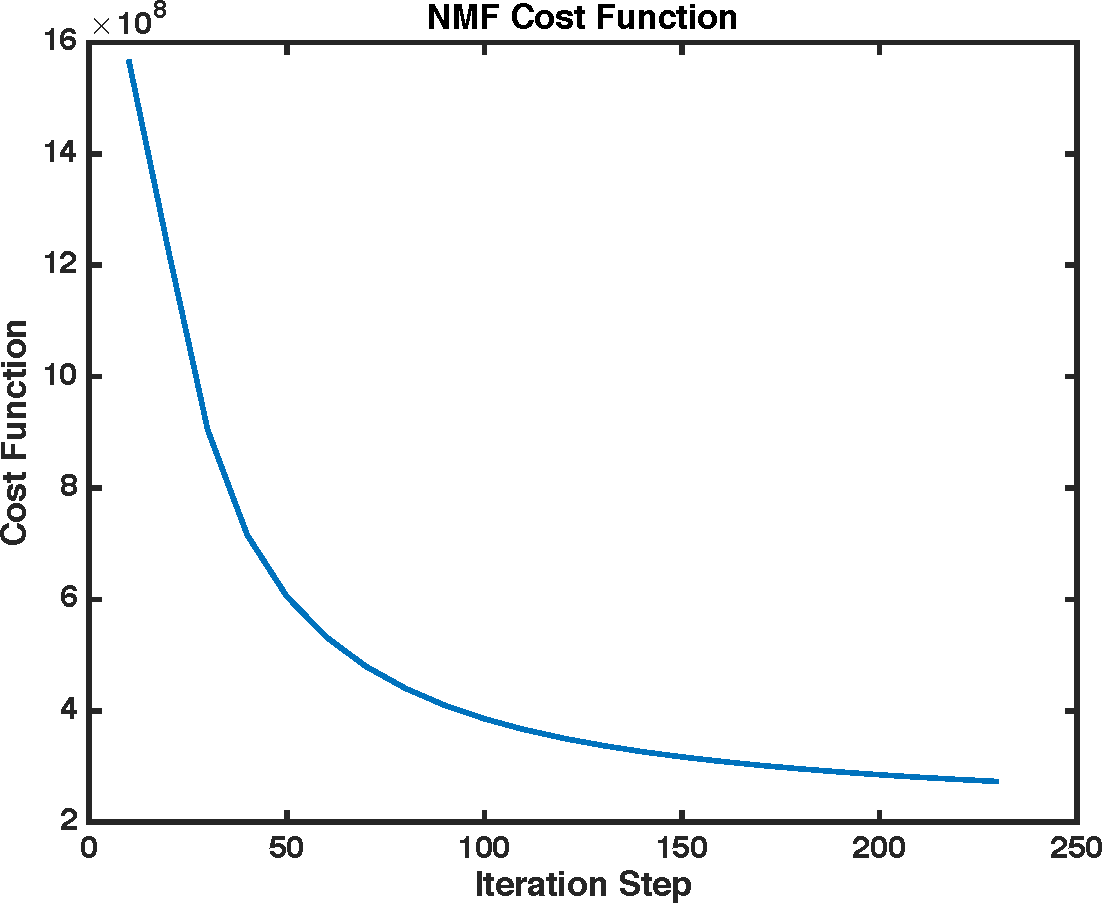
\includegraphics[width=\MyFactor\textwidth]{Img/nmf_cost.pdf} \captionof{figure}{NMF的惩罚函数下降曲线 \\ x坐标:迭代次数, y坐标 惩罚函数\ref{nmf_cost}}
}
\end{minipage}
\medskip
\end{center}

\subsection{NMF的在ORL测试集的投影基底}
以下是使用ORL数据集120张图片作为基底(40个人,每人三张),选择结果的前64张图片得到的特征基底.只选择120个图片用来计算是因为NMF的计算速度较慢.
\begin{center}
\begin{minipage}[t]{\linewidth}
%\label{fig:main}
\center
{
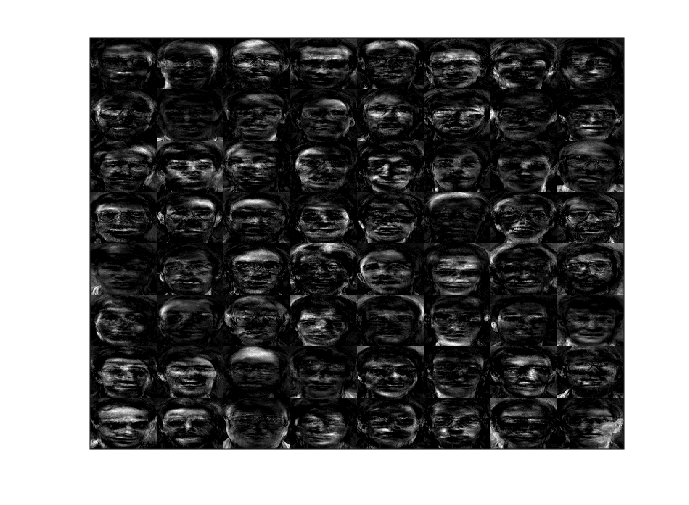
\includegraphics[width=\textwidth]{Img/nmf_base.png} \captionof{figure}{NMF的在ORL测试集的投影基底}
}
\end{minipage}
\medskip
\end{center}


由于NMF基底不是正交的,使用了\textit{Matlab}函数中\textit{Pinv()}函数计算了伪逆来投影.
\section{ICA}
\subsection{ICA的思想和计算方法}
ICA被有些文献称为PCA的延伸,对于PCA,它使得样本之间的二阶统计量最小化,对于ICA,它使得样本中二阶及以上的统计量最小化,也就是使得样本之间独立.所谓的独立性,指的是 \begin{equation}
		f_s(s) = \prod_i f_{s_i}(s_i)
	\end{equation}
	其中$f_s$是信号的分布密度函数.

本章节所主要依据的文献是\cite{icafordummies, draper2003recognizing, vaseghi2006principal, langlois2010introduction, hyvarinen2000independent, awasthyanalysis, khaparde2008fastica}\newline

ICA试图解决如下问题:\begin{equation}
	x = As
\end{equation}
其中,已知的只有混合后的信号x,A为混合信号时的权值,s为信号源.ICA试图在未知A的情况下求得s.

为了进一步简化问题,ICA作出如下假设,假设x的长度与s的长度一致.也就是,混合信号的数量和信号源的数量一致.这使得A成为一个方阵.同时,也使得A可逆,记其逆矩阵为W.那么有下列关系:
\begin{equation}
	\label{ICA:SourceDecompose}
	s=Wx
\end{equation}
ICA的核心就是在估计W来更好的得到s.\newline

ICA的推导中对变量有一定的要求,需要进行一些预处理,这些操作有:
\begin{enumerate}
	\item{中心化} 该步使用公式\ref{Centering},使得$ \tau_i$平均值为0
	\item{白化} 该操作使得各个变量之间无关(uncorrelated)并且方差为1.也就是满足\ref{pca:corr}.该步操作可以在输入样本上执行PCA来完成.
\end{enumerate}
如此可见,PCA处理过的结果满足ICA的要求,因此PCA常常被用来ICA的预处理操作.PCA处理过的结果不仅满足ICA的预处理要求,并且PCA预先对样本进行了降维操作,简化了ICA的运算.\newline

白化后,开始按照\label{ICA:SourceDecompose}来进行分解.目前共有两类不同思想的ICA实现方法,分别是\textit{FastICA}和\textit{InfoMax}.下面进行简要介绍.
	\paragraph{FastICA}	\textit{FastICA}使用\textit{Negentropy}来表征变量间的独立程度,\textit{Negentropy}的定义为
	\begin{equation}
		J(y) = H(ygauss) - H(y)
	\end{equation}
	J是一个非负数,表征了参数的非高斯性,当为0时,为高斯分布.
	
	可使用\textit{Kurtosis}来近似\textit{Negentropy},\textit{Kurtosis}公式为
	\begin{equation}
		kurt(y) = E(y^4) - 3(E(y^2))^2
	\end{equation}
	E(y)代表y的期望值(下同)
	
	近似后的结果为
	\begin{equation}
		J(y) \approx \frac{1}{12}E(y^3)^2+\frac{1}{48}kurt(y)^2
	\end{equation}
	并可被进一步近似为
	\begin{equation}
		J(y) \approx \Sigma^p_{i=1}k_i[E(G_i(y)) - E(G_i(v))^2]
	\end{equation}
	当仅仅使用一个函数G时,可进一步近似为
	\begin{equation}
	\label{ica_g}
		J(y) \propto (E(G(y)) - E(G(v)))^2
	\end{equation}
	
	G是可以被定义的,\cite{hyvarinen2000independent}中给出了比较有用的形式:
	\begin{multicols}{2}
		\begin{equation}
			G_1(u) = \frac{1}{a_1}log(cosh(a_1u))
		\end{equation}
	
		\begin{equation}
			G_2(u) = -exp(-u^2/2)
		\end{equation}
	\end{multicols}
	其中的$a_1$是常数, $1 \leqslant a_1 \leqslant 2$.\newline


	而\textit{FastICA}算法就是一种类似牛顿法的使用梯度下降法(Gradient Descent)方法来逼近J最大值的方法. 
	
	\paragraph{InfoMax}
	\textit{FastICA}从信息论的角度,来求得最大的\textit{Negentropy},而\textit{InfoMax}则从最小化\textit{Mutual information}的角度出发.
	
	\textit{Mutual information}的定义是
	\begin{equation}
		I(y_1,y_2,...,y_m) = \Sigma_{i=1}^m H(y_i) - H(y)
	\end{equation}
	\cite{hyvarinen2000independent}中,推导得到,经过ICA预处理过程的变量,满足\begin{equation}
			I(y_1,y_2,...,y_m) = C - \Sigma_iJ(y_i)
		\end{equation}
		其中C是一个常数.
		
		由此可见,I和J是相关的变量.而\textit{FastICA}中J的最大化和\textit{InfoMax}中I最小化的求解有相同的目的.\textit{InfoMax}本身是一种利用梯度下降法来逼近I的最小值的方法.
	
	\paragraph{FastICA 和 InfoMax的比较}
	从\cite{draper2003recognizing}得到,其实,虽然\textit{FastICA}和\textit{InfoMax}形式不同,但是差别并不大.\cite{draper2003recognizing}还索引了之前的一些经验性的比较,发现结果并无太大差别.\newline
	
	本项目中,使用了\cite{fastica25}的\textit{FastICA}实现方法.	
	\paragraph{ICA的缺点} 同时,这些引用文献也多提到了ICA的实际应用上的一些缺点,总结如下
	\begin{itemize}
		\item ICA计算的结果与原本信号源$s$的结果的顺序被不一致
		\item ICA做了非高斯分布的假设.当高斯分布时,无法进行ICA运算
		\item ICA计算出的分量是独立平行的,丢失了方差,无法看出权重
	\end{itemize}

\subsection{ICA的主要应用}
需要指出的,人脸图像分解并非ICA的主要应用场所,ICA的应用最初产生于盲源分离(Blind Source Seperation, BSS), 下面将对ICA在盲源分离的应用做一些简要介绍,并给出ICA在人脸图像分解直觉上的动机.\newline

经过上一章节的介绍,ICA可以在混合信号$x$中解混,分析出s,以下是ICA作用于一维的变量中的效果:
	\paragraph{ICA作用于一维的变量}	
	以下是ICA用于解混3个信号的示意,第一栏是原始信号,第二栏是混合后的信号,第三栏是解混后的信号,混合信号的A是
	\begin{center}
	\captionof{table}{随机混合矩阵A}
	\begin{tabular}{|l|l|l|}
\hline
0.037195&0.58635&0.80667\\\hline
0.55504&0.17859&0.091525\\\hline
0.67324&0.41986&0.07831\\\hline
\end{tabular}
\end{center}

同时,\ref{ica_g}中的方程$G()$取形式$g(u)=tanh(a1*u)$,终止条件J的阈值取为默认值0.0001.

\begin{center}
\begin{minipage}[t]{\linewidth}
\center
{
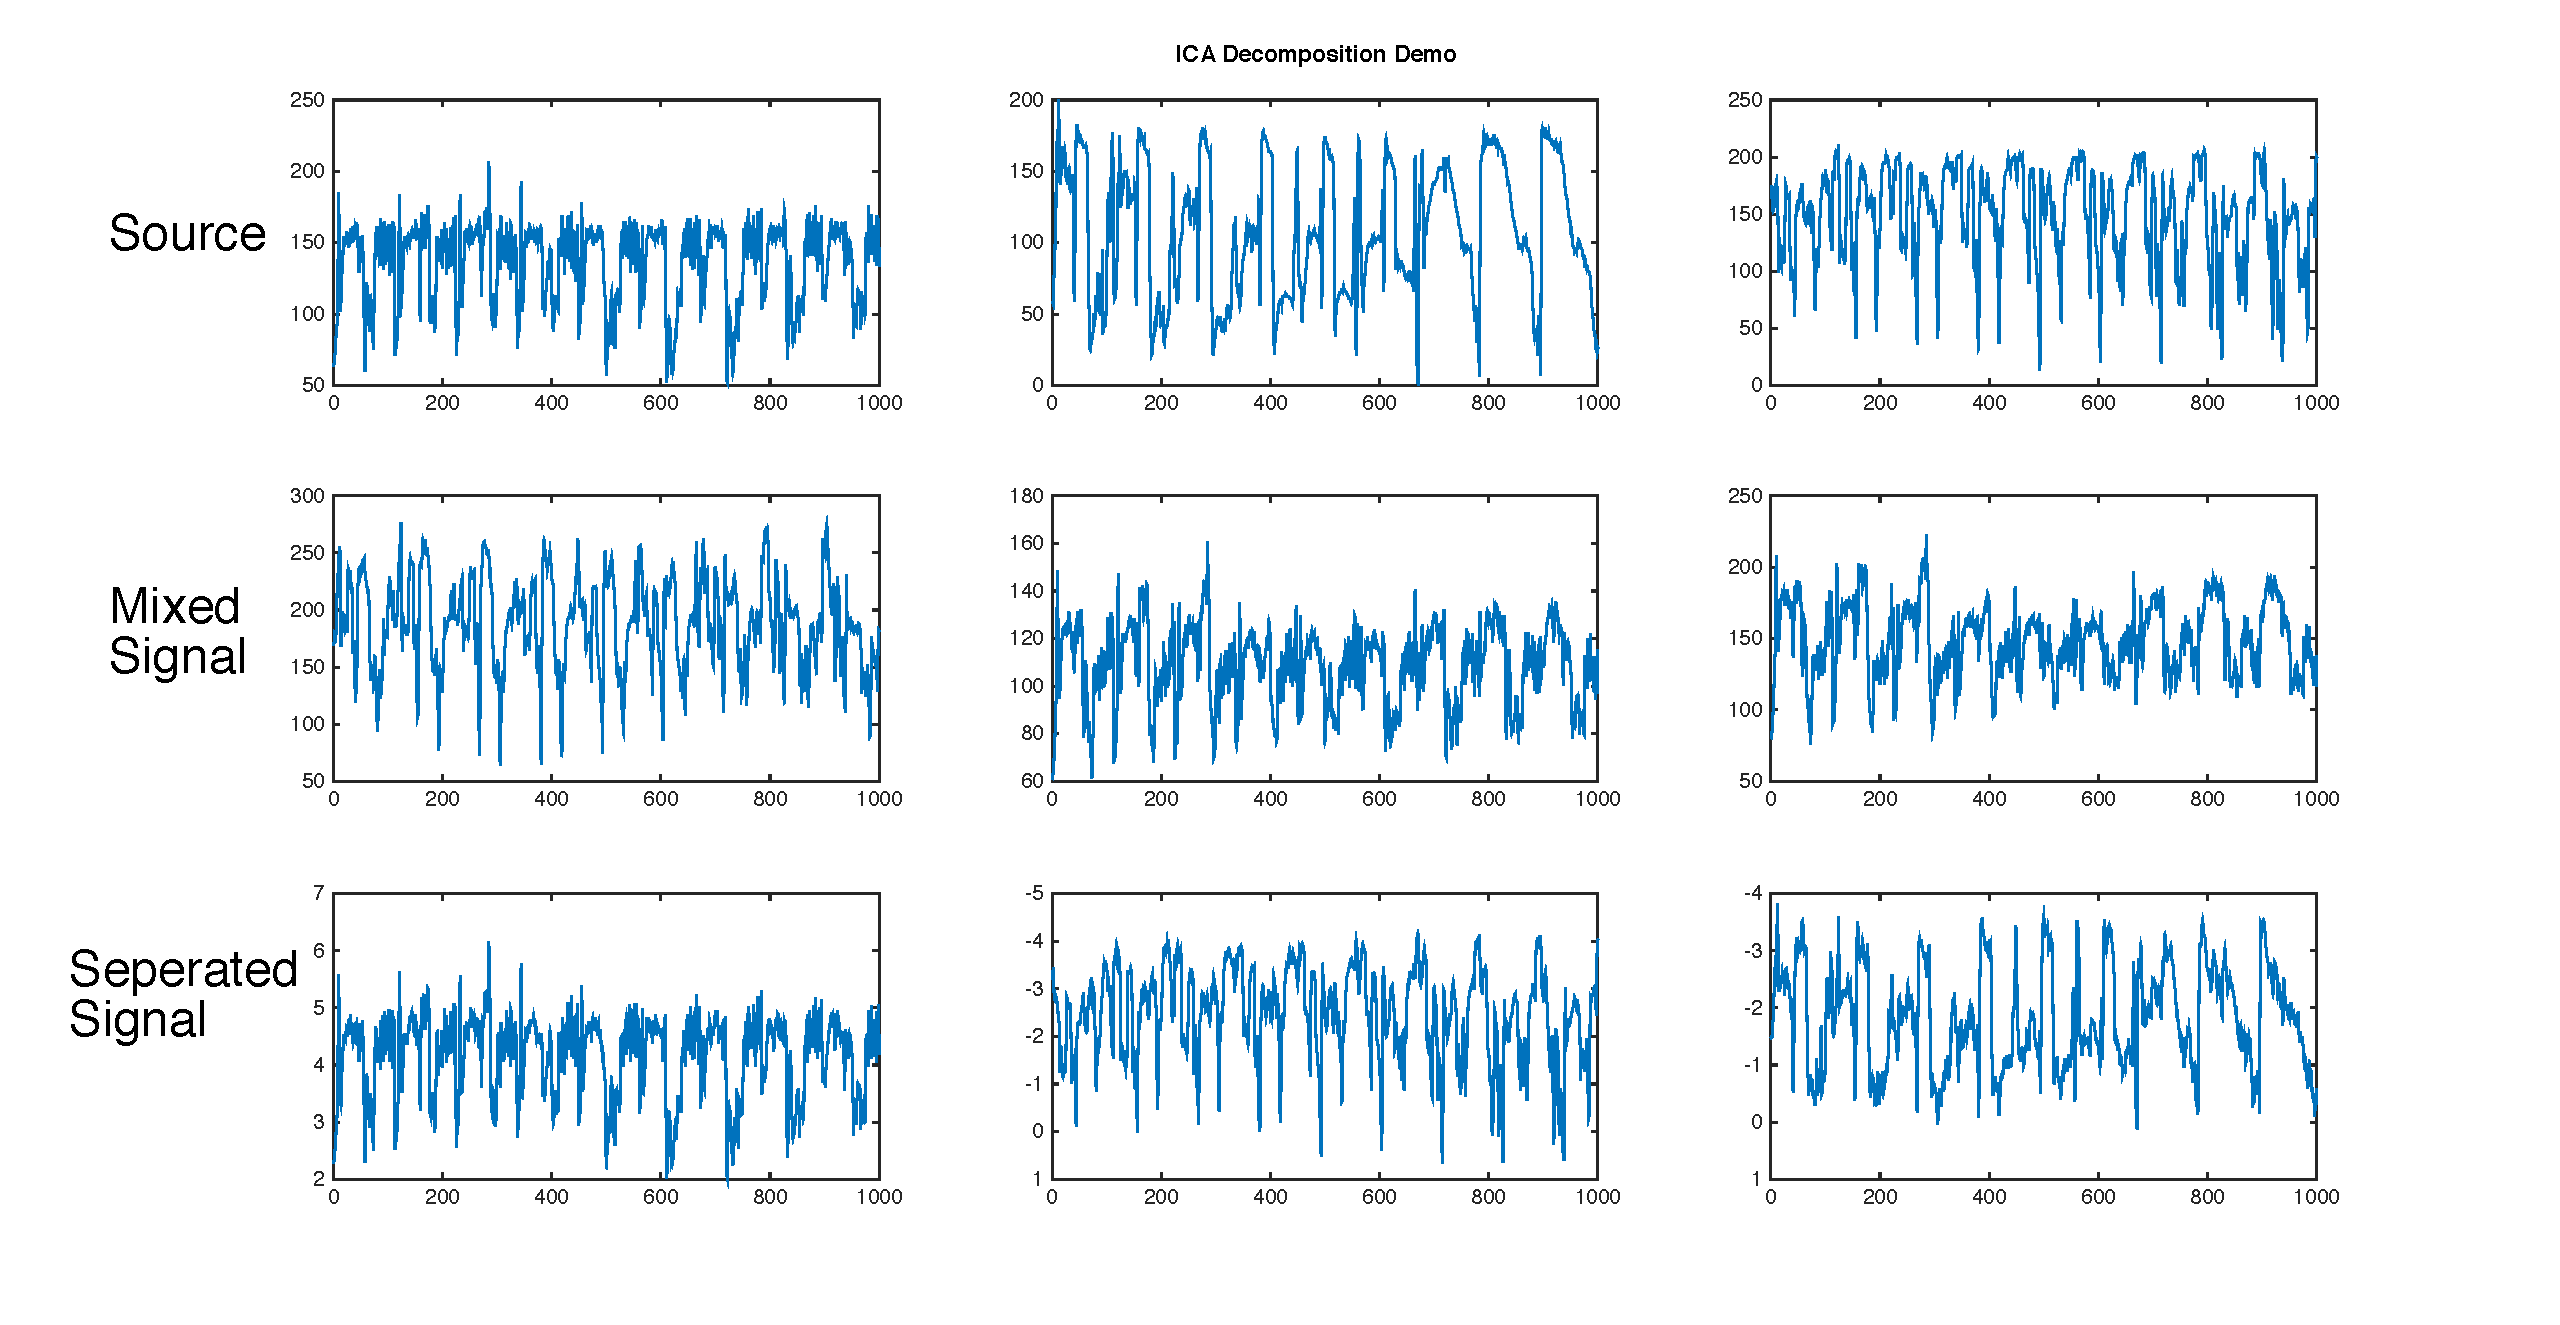
\includegraphics[width=\textwidth]{Img/ica_decom.pdf} 
\captionof{figure}{ICA解混示意\\ 由于ICA使相位改变了,解混信号被翻转了}
\label{fig:icadecom}
}
\end{minipage}
\medskip
\end{center}

可以明显看到,信号1和解混后信号1,信号2和解混后信号3,信号3和解混后信号2是比较相像的.说明ICA已经成功从第二栏的输入信号中分解出了原始信号.当然了,由于ICA作用于矩阵的缺点,解混信号的顺序,相位都被打乱了.
\paragraph{ICA作用于二维的变量}
实际了,上述3个长度1000的随机向量是3张$112 \times 92$图片的前1000元素,而ICA实际上也是作用于这3张混合后的图片的,以下是分解的结果:

\begin{center}
\begin{minipage}[t]{\linewidth}
\center
{
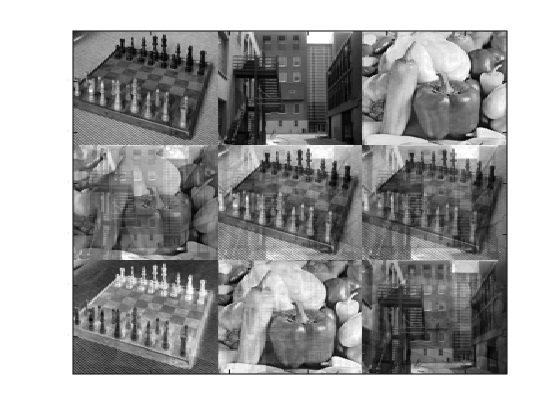
\includegraphics[width=\textwidth]{Img/ica_decom2.png} \captionof{figure}{2D ICA解混示意\\ 由于ICA使相位改变了,解混信号被翻转了}
	\label{fig:icadecom2}
}
\end{minipage}
\medskip
\end{center}
图片放置的顺序和\ref{fig:icadecom}一样,可见,ICA成功得从第二栏混合后的向量中分解出了第一栏的图片.\newline

从此就引出了ICA作用于人脸图像的动机了,如果输入人脸图像是\ref{fig:icadecom2}的第二栏图像,我们也用相同的方法来分解,必然能得到一些分解的结果.当假定人脸图像是有若干独立的变量线性组合而成的,自然地,我们就得到了第三栏这些分量.而这些分量具有相互独立的性质,本项目假定人脸图像就是由这些分量组合而来的,并以其作为投影的基底.


\subsection{ICA的在ORL测试集的投影基底}
以下是使用ORL数据集120张图片作为基底(40个人,每人三张),选择结果的前64张图片得到的特征基底.只选择120个图片用来计算是因为ICA的计算速度较慢.
\begin{center}
\begin{minipage}[t]{\linewidth}
%\label{fig:main}
\center
{
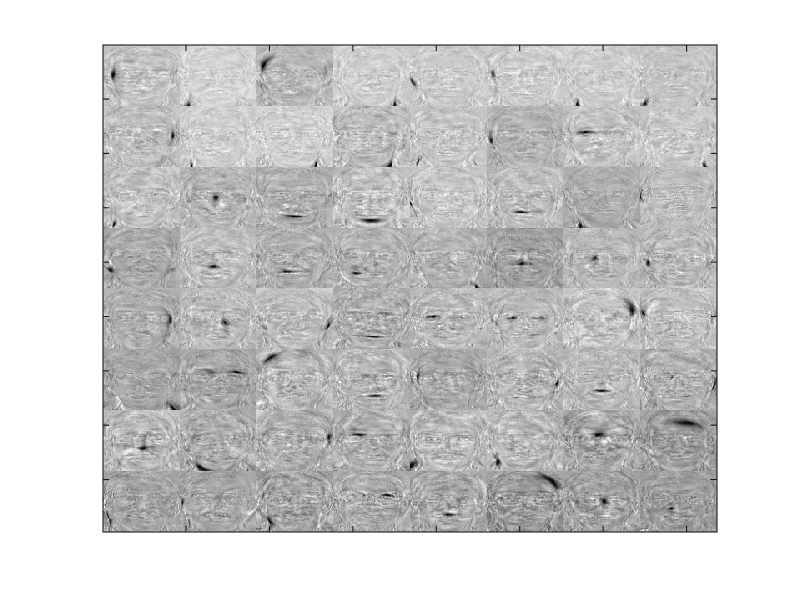
\includegraphics[width=\textwidth]{Img/ica_base.png} \captionof{figure}{ICA的在ORL测试集的投影基底}
\label{fig:ica_base}
}
\end{minipage}
\medskip
\end{center}
由于ICA基底不是正交的,使用了\textit{Matlab}函数中\textit{Pinv()}函数计算了伪逆来投影.



需要指出的是,ICA分解结果具有较强的稀疏性,因此也被用来压缩图像.这在\ref{fig:ica_base}中,可以看出大部分特征脸的部分都接近于0(近乎白色或者灰色)

%\section{DCT}
%在之前的实践中,笔者发现实际上任何图片的较为短小的并且与图片有较大联系的相关向量都可以被当做特征向量.这里,本项目从频域的角度出发,提取了图片的频域基频特征.
%\section{更多的基底}
%除了这些方法,还有很多其他的方法.\cite{de2010face}列出了更为详尽的列表,限于项目时间的限制,并没有深入研究这些所有的算法,仅仅尽可能的通过\textit{SciKit}工具包来列出相同测试样本下的基底.
%	\begin{itemize}
%		\item Kernel PCA
%		\item Weighted PCA
%		\item Linear Discriminant Analysis (LDA)
%		\item Kernel LDA
%		\item Semi-supervised Discriminant Analysis (SDA)
%		\item Neural Network based methods
%		\item Multidimensional Scaling (MDS)
%		\item Self-organizing map (SOM)
%		\item Active Shape Models (ASM)
%		\item Active Appearance Models (AAM)
%		\item Gavor wavelet transforms
%		\item MMSD, SMSD
%	\end{itemize}

\section{相关实验}
参见\ref{sec:comp_global}.




	
%\chapter{基于局部的特征提取算法}
\label{cha:local}
在上一节的学习过程中,笔者渐渐感觉到计算算子对人脸识别,分类系统的影响非常大,毕竟,人脸图像被分解后,仅仅由一个很短的向量来表示,那该编码系统对样本的区分程度很大程度上就能决定后续分类系统的性能.因此,我渐渐发现了基于局部的特征提取算法,它们有些具有\textit{Content Awareness}的特性,对背景噪声有一定的区分能力,并且可以精细的比较样本的细节之处,因此可以达到精确的识别性能.本章节以SIFT算子为例做介绍.

\section{SIFT}
\subsection{SIFT的原理}
本章节主要基于\cite{lowe2004distinctive, issolah2013sift, juan2009comparison, siftopencv, siftvlfeat, siftubc,lowe1999object},在Matlab中使用了\cite{siftvlfeat}实现的SIFT算法. \newline

SIFT算子的计算方法共分4步.
\begin{enumerate}
	\item SIFT首先构建一系列DoG(Difference-of-Gaussian)金字塔.并在其上计算极值,作为该层空间上的特征点.具体的计算方法是求得所有满足在其$3 \times 3$临域上为最大值或最小值的点. 

	 	\begin{center}
		\begin{minipage}[t]{\linewidth}
		%\label{fig:main}
		\center
		{
		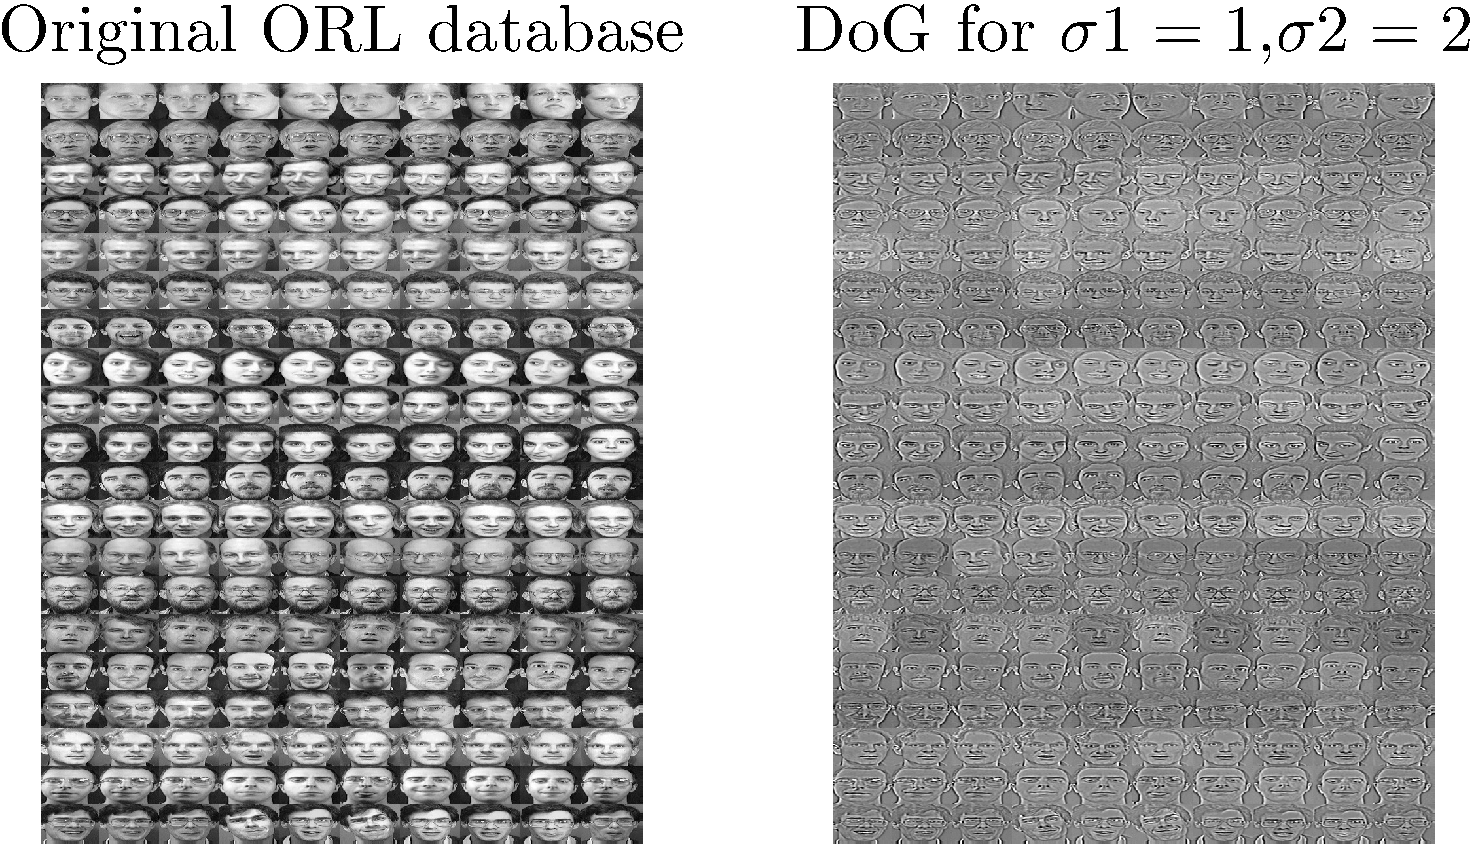
\includegraphics[width=\textwidth]{Img/c3/dog_demo} \captionof{figure}{DoG滤波示意图,DoG图像采用了和输入图像相同的尺度}
		}
		\end{minipage}
		\medskip
		\end{center}
	
	\item 当每层的特征点被计算出来后, SIFT计算该层求得的特征点是否在解析度更大的一层上也满足为最大值或最小值.只有一直满足该特性的点才能被下一步运算.运算结束后,SIFT再一步过滤掉因噪音,边界而被误判为特征点的点.SIFT空间保留了差值运算中特征点相对最初一层邻域的尺度,以及特征点的位置作为特征点的描述.
	\item SIFT在计算出特征位置上每隔$10^\circ$的梯度,并选择梯度最大及三个以内的大于某阈值梯度的方向为该特征位置的方向.经过以上三步,SIFT计算出了输入图片的特征点.
	
		 \begin{center}
		\begin{minipage}[t]{\linewidth}
		%\label{fig:main}
		\center
		{
		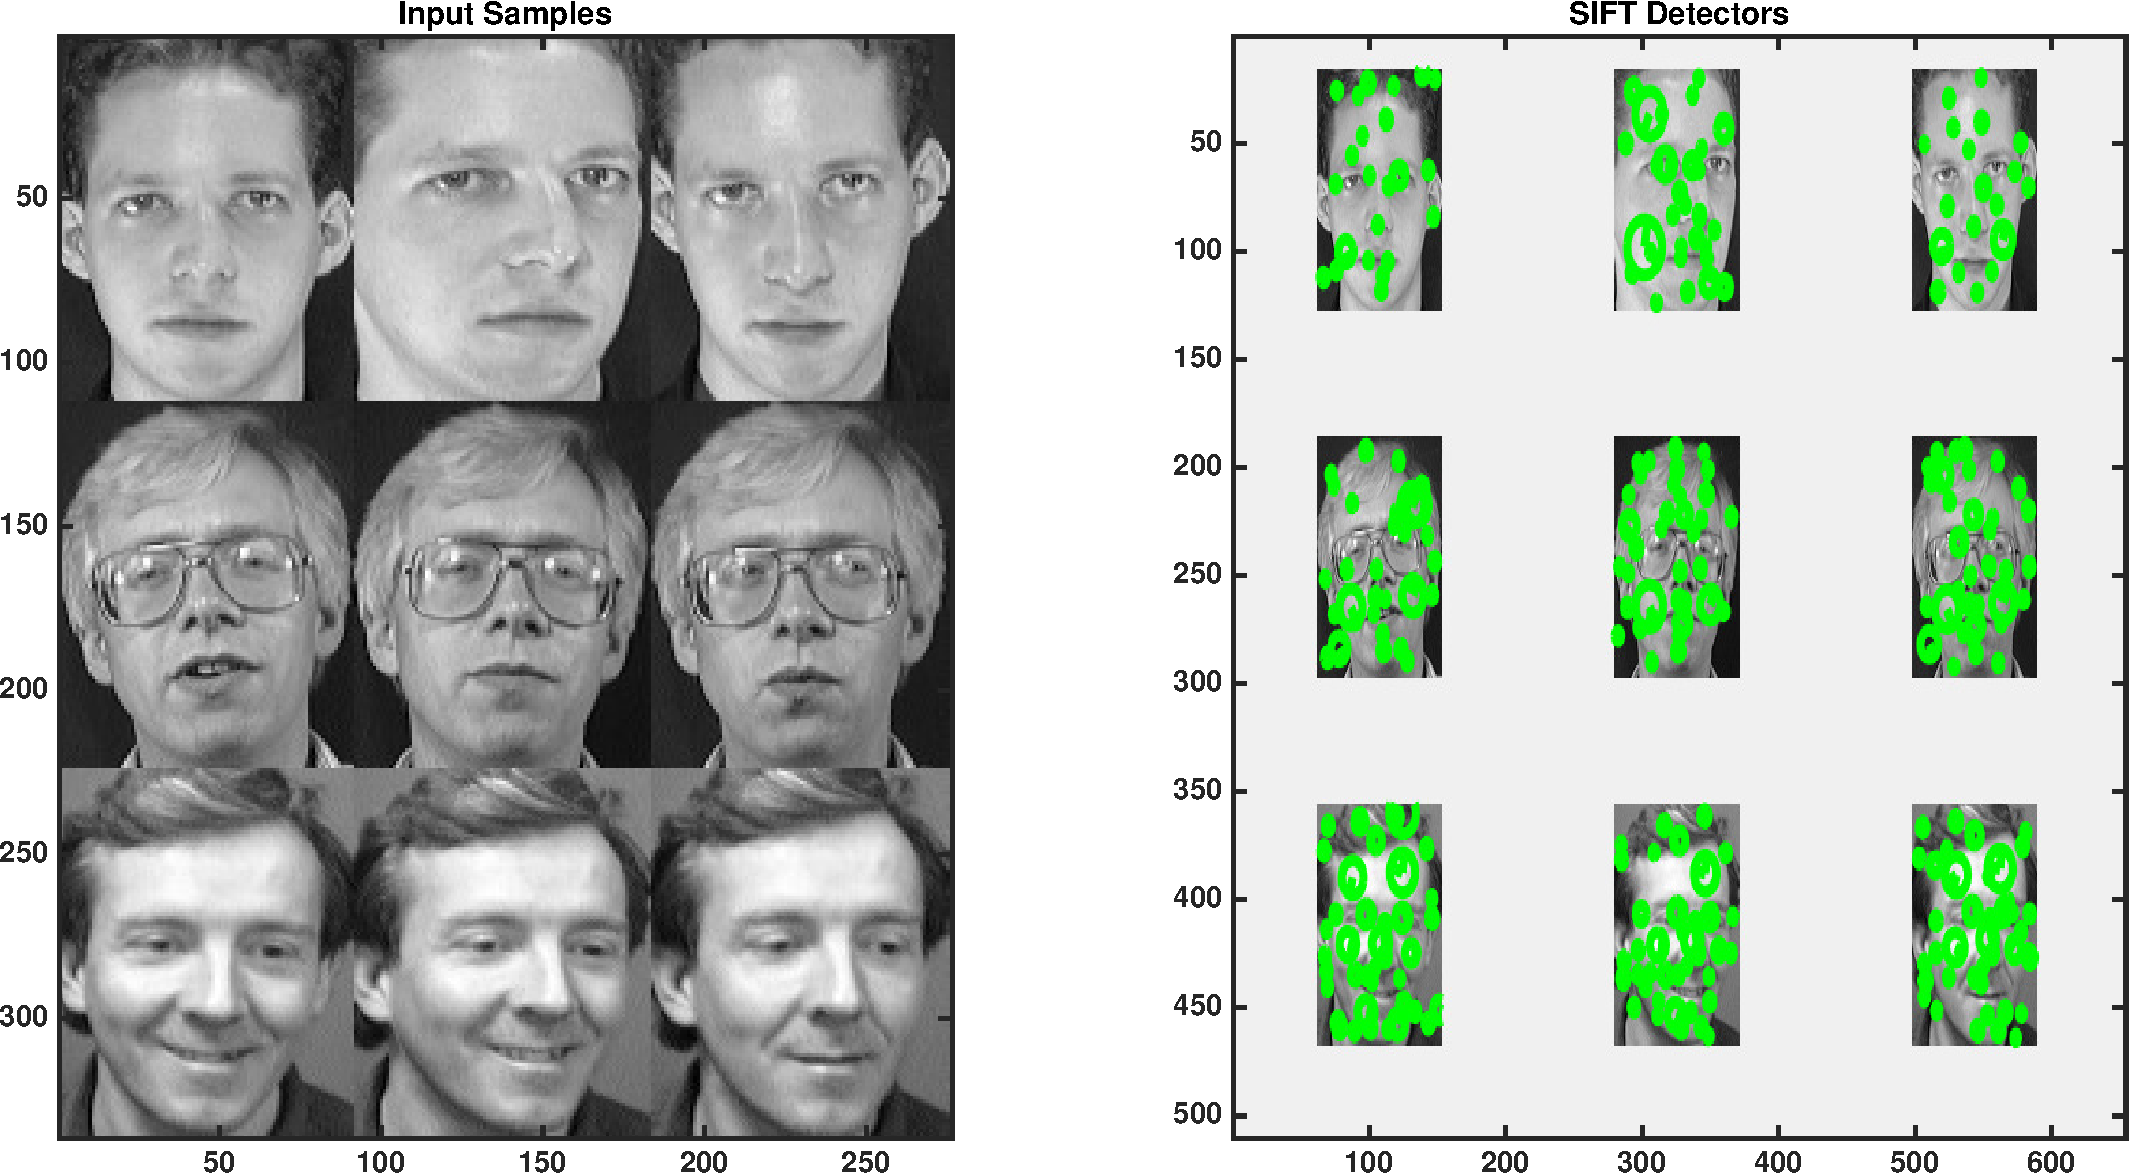
\includegraphics[width=\textwidth]{Img/c3/sift_detectors.pdf} \captionof{figure}{SIFT特征点示意}
		}
		\end{minipage}
		\medskip
		\end{center}
	\item 最后一步是对特征点的描述,SIFT采用一个$N_\theta \times N_x \times N_y$(通常为$8 \times 4 \times 4$,其中$\theta$,$x$,$y$取不同的值,并分别在特征空间上计算梯度)的向量(又称HoG, Histogram of Gradients)来描述该特征点的性质.在\textit{SIFT-PCA}算法采用了另一种方法.
		\begin{center}
		\begin{minipage}[t]{\linewidth}
		%\label{fig:main}
		\center
		{
		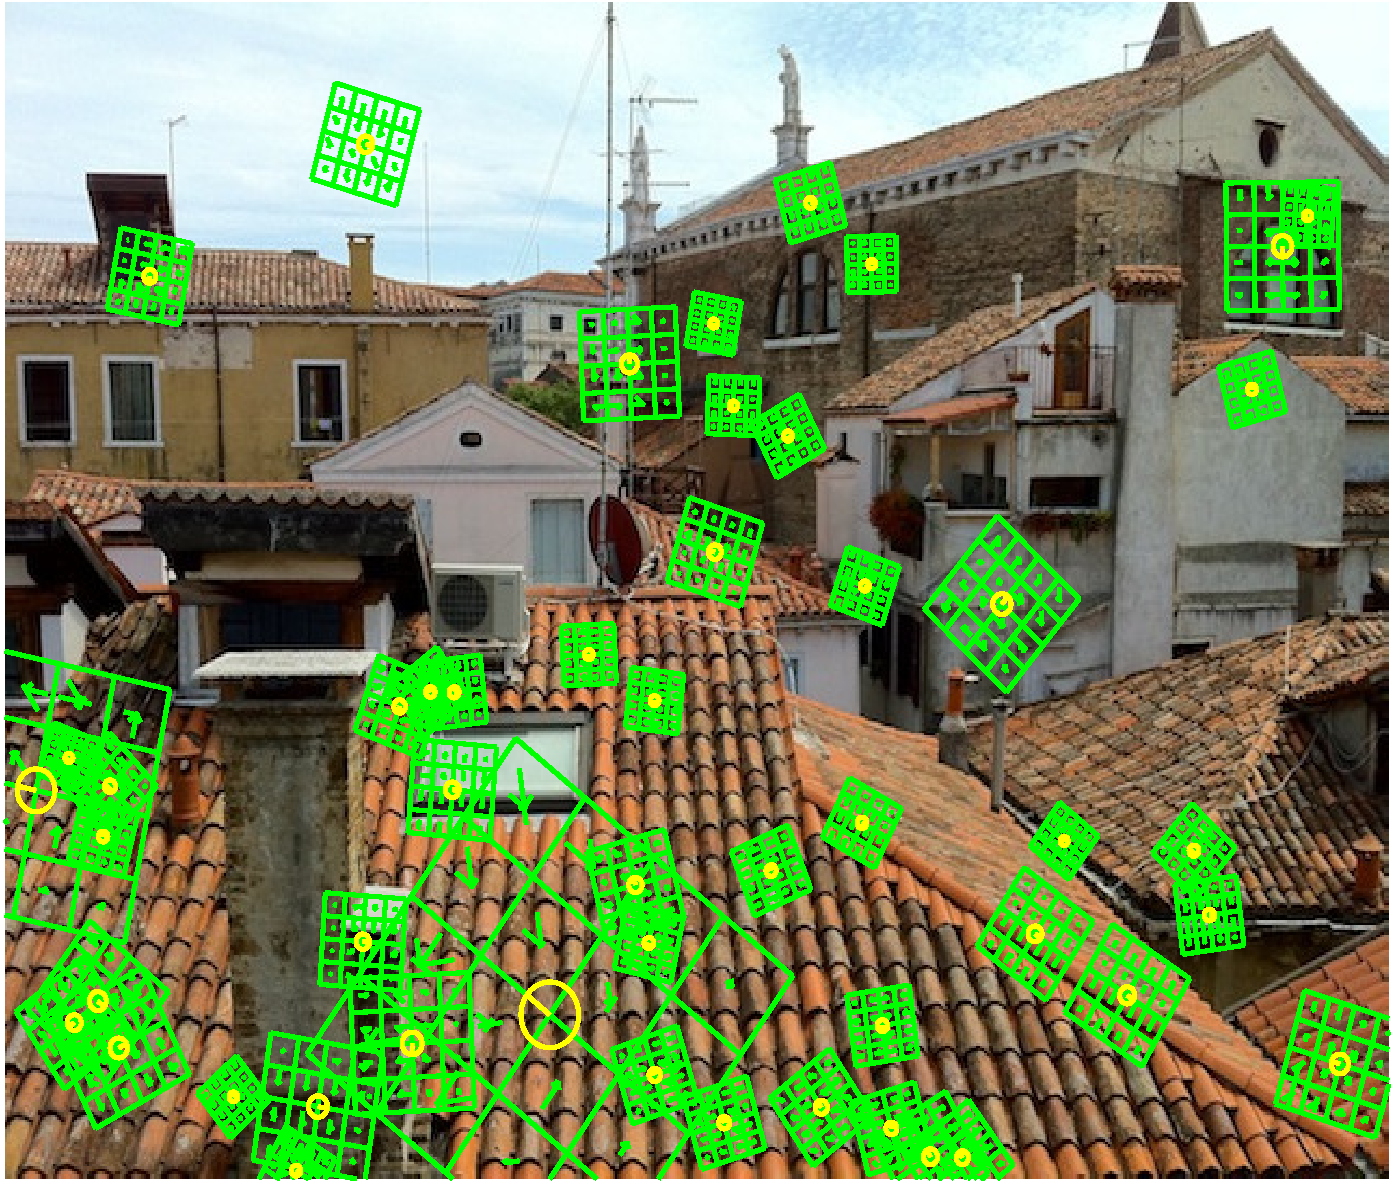
\includegraphics[width=\MyFactor\textwidth]{Img/c3/sift_demo} \captionof{figure}{SIFT特征点的描述,来源\cite{siftvlfeat}}
		}
		\end{minipage}
		\medskip
		\end{center}
		上图就是通常的SIFT描述的表示方法,可见,它是由一个$4 \times 4$的方阵表示的,分别表示了特征点所确定的特征空间的x,y取值的梯度.而每个方阵内部又由一个8个方向变化长度的向量表示,向量的长度表示了在该方阵x,y确定的位置上,不同$\theta$下的梯度大小.总计共有128($8 \times 4 \times 4$)个向量来描述特征点所对应的特征空间.
	\end{enumerate}



\subsection{SIFT-PCA算法}
由于SIFT运算结果过长,笔者实现了SIFT-PCA算子\cite{ke2004pca},它是一种采用块压缩技术的基于SIFT的1-3步的方法.具有可调节的长度.

	 	\begin{center}
		\begin{minipage}[t]{\linewidth}
		\center
		{
		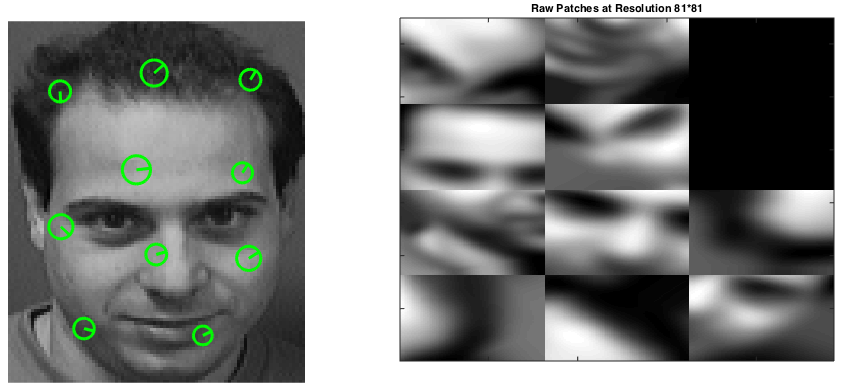
\includegraphics[width=\MyFactor\textwidth]{Img/c3/sift_raw_patch2} 
		\captionsetup{justification=centering}
		\captionof{figure}{SIFT特征点和对应的特征空间示意\\ 为了演示方便,图像中特征点对应$81 \times 81$的邻域,而实际计算中特征点对应$41 \times 41$的邻域}
				\label{fig:sift_patches}
		}
		\end{minipage}
		\medskip
		\end{center}
	
	它的具体步骤是建立在SIFT算法的1到3步上的,在标准特征位置所描述的空间上:
	\begin{enumerate}
		\item SIFT-PCA算法首先计算该空间的水平,竖直两个梯度空间(本文中使用了Sobel方法).同时,为了避免边界梯度的骤增,边界的梯度被剔除了.
			
		\begin{center}
		\begin{minipage}[t]{\linewidth}
		\center
		{
		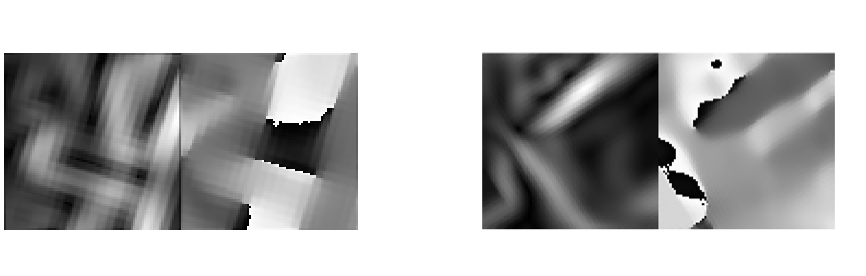
\includegraphics[width=\MyFactor\textwidth]{Img/c3/gradient.png} 
		\captionsetup{justification=centering}
		\captionof{figure}{水平,竖直两个梯度空间示意\\ 左:使用Sobel算子,右:使用prewitt算子\\ 计算\ref{fig:sift_patches}第一张图片的特征空间}
		}
		\end{minipage}
		\medskip
		\end{center}
		
		\item SIFT-PCA计算多张图片多个特征点上的梯度空间,并且使用PCA对其进行降维运算
		\item 当新输入空间时,SIFT-PCA使用标准SIFT算法提取特征点及特征点对应的空间,计算出对应空间的水平,竖直梯度空间后,对这两个空间使用上一步的基底降维.坐标就是SIFT-PCA对特征点对应的描述
	\end{enumerate}
	本文实现中,使用了100个人所提取出的特征梯度空间用作SIFT-PCA基底的学习,并在3600左右的特征向量中取前20个作为PCA降维后的特征向量,降维后的前20特征值占据了约60\%的特征值,下面是PCA的特征值绘制:
	
			\begin{center}
		\begin{minipage}[t]{\linewidth}
		%\label{fig:main}
		\center
		{
		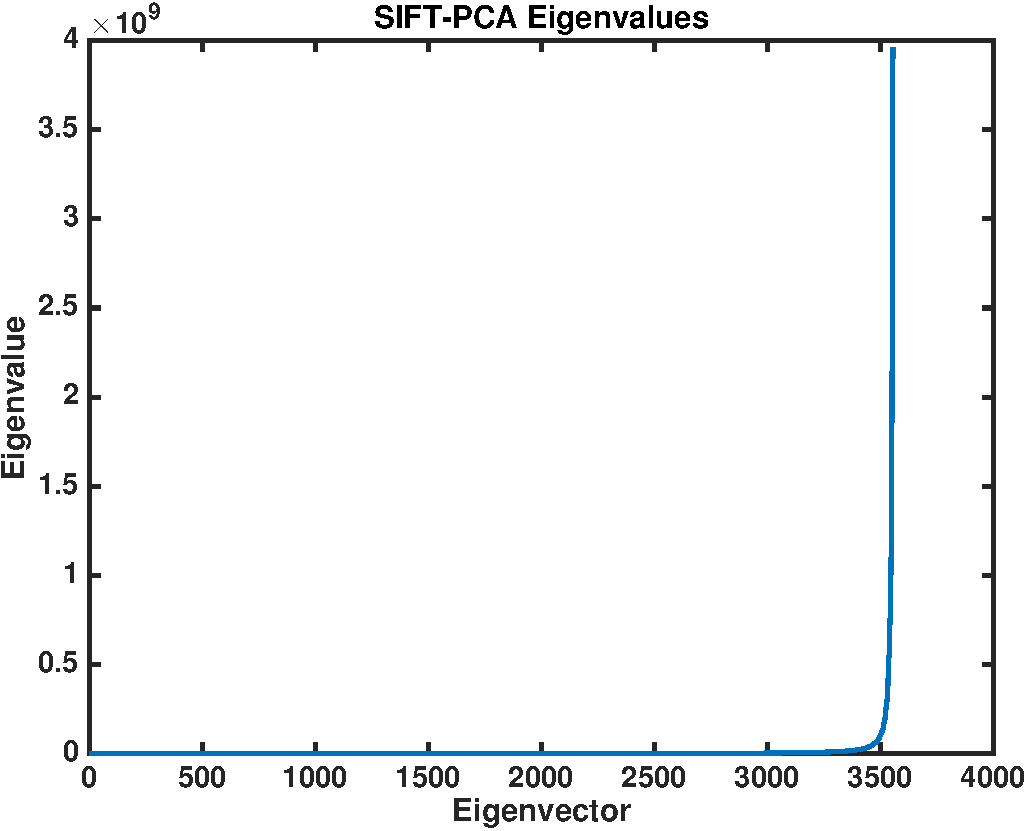
\includegraphics[width=\MyFactor\textwidth]{Img/c3/sift_pca_eigen} 
		\captionof{figure}{PCA的特征值}
		}
		\end{minipage}
		\medskip
		\end{center}
		
	经过SIFT-PCA后,SIFT算法原长度为128位的HoG特征描述就被PCA压缩为20位了.
		

\subsection{SIFT的编码方法}
由于SIFT算子是\textit{Content Aware}的,其特征提取的结果是由若干个特征点确定的特征空间来描述的.由于特征点的数目不确定,所以特征向量的总长度并不固定.这对后续的分类算法并不友好.因此,SIFT的结果大都被编码了,编码方法通常有以下的方法.\cite{chatfield2011devil}
	\paragraph{BoF: Bag-of-Features}
	BoW(Bag-of-Word)是文本处理中的手段,是指文本处理中,对文本的词汇分布作直方图的手段.也就是将该文本内所有出现过的词汇统计出来,并计算它们的出现频率.\newline
	
	BoF或BoVF(Bag-of-Visual-Features)是该BoW在局部特征提取的延伸手段,它统计了局部特征的特征点,当输入新样本时,样本在这些特征点的分布图就是它的全局特征.具体说来,BoF共分两步: \newline
	
	第一步是在输入样本之前,求得特征点分布重心的过程,它并不需要在输入样本时计算,可以离线提前求出.它的具体过程可以是:
	\begin{enumerate}
		\item 准备一些样本图像,并求得它们SIFT特征空间描述的全集
		\item 在这个全集上执行\textit{kmeans}运算,k值取值就是重心的数量,也就是之后全局样本的维度.并记录下重心的取值(也被成为\textit{Visual Vocabulary}).
	\end{enumerate}
	第二步是求得输入样本坐标的过程,它的过程可以是:
	\begin{enumerate}
		\item 取得样本的SIFT特征空间描述
		\item 对于每个描述,求得它最近重心,并被归到那一类里去
		\item 归类后,可以得到各个重心被归类的描述数目,而他们的分布就是该图像的BoF
	\end{enumerate}
	
	下面是结合标准的SIFT算法,分别取聚类个数为40,100,300,1500,3000的距离矩阵,计算BoW的样本有120张,总共提取了约4500个特征点,
	
		\begin{center}
		\begin{minipage}[t]{\linewidth}
		%\label{fig:main}
		\center
		{
		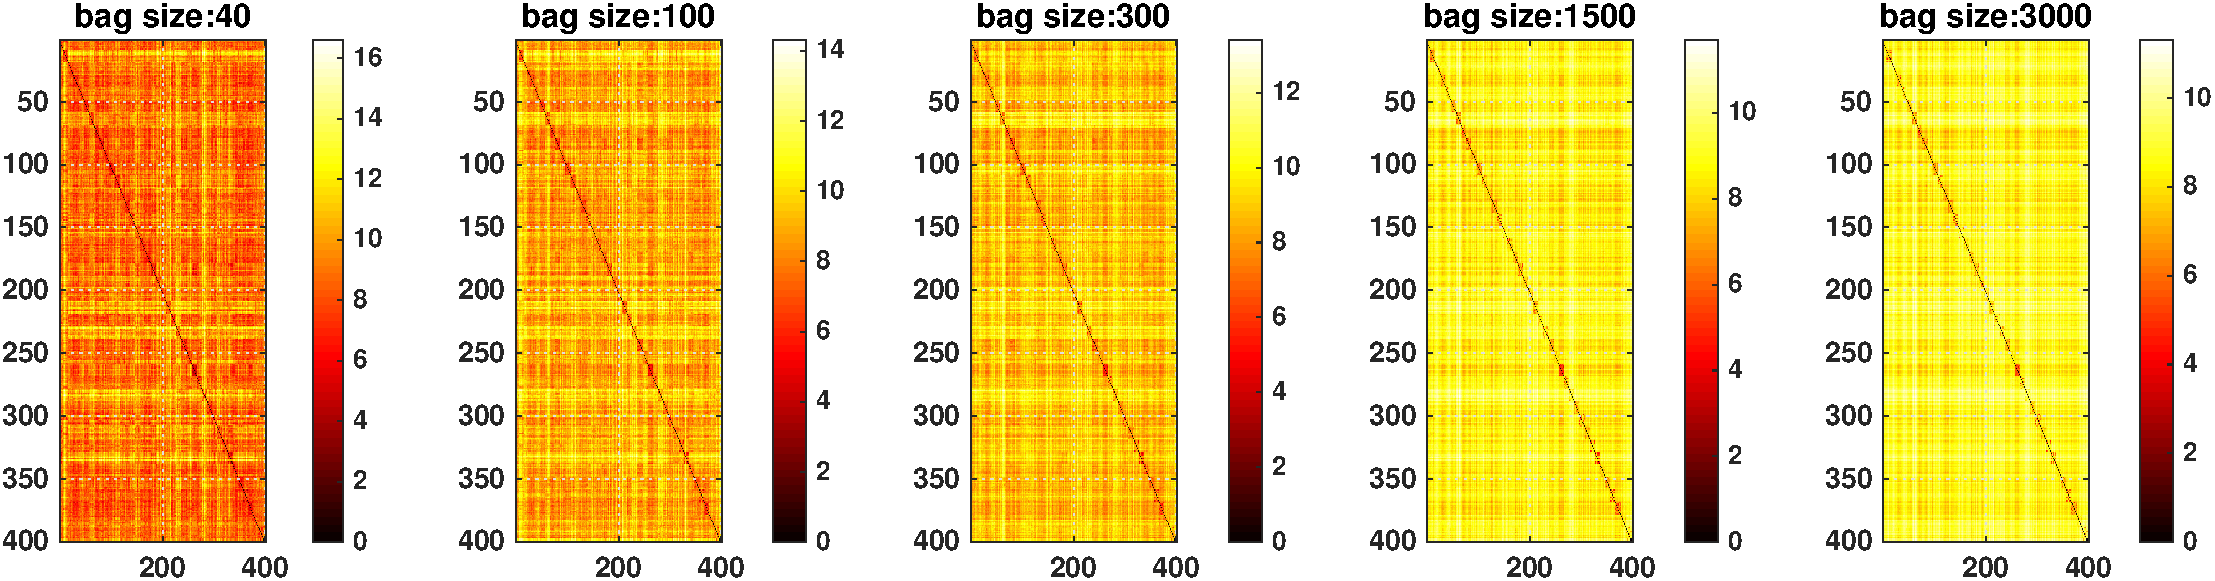
\includegraphics[width=\textwidth]{Img/c3/sift_bow_iter} 
		\captionof{figure}{BoW距离矩阵}
		}
		\end{minipage}
		\medskip
		\end{center}
		
		由此可见,BoW对人脸图像的泛化能力并不好,具体表现为类间距离和类内距离差别不大.而BoW的主要应用场所在于场景识别,对于人脸识别,由于人脸大都大同小异,所以聚类梯度的方法就不是很适用.
	\paragraph{在固定点计算描述}
	由于人脸图像的分布大体一致,该过程没有对特征的描述来分类,而是对特征的位置进行了分类,并且在固定的位置上计算它的描述.它的过程也分为两步,分别是离线的计算特征的位置,和在线的在固定的位置上计算特征的描述\newline
	
	第一步是离线计算特征点的位置,
	\begin{enumerate}
		\item 首先准备一些样本图像,并求得它们特征空间位置的全集
		\item 在这个四维空间(位置,尺度还有角度)的全集上执行\textit{kmeans}运算,k值得取值就是特征点的个数
	\end{enumerate}
	
				\begin{center}
		\begin{minipage}[t]{\linewidth}
		%\label{fig:main}
		\center
		{
		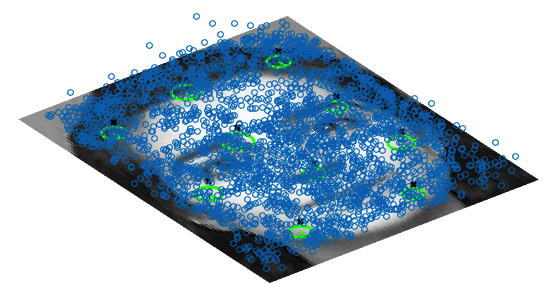
\includegraphics[width=\MyFactor\textwidth]{Img/c3/sift_face_kmeans} 
		\captionof{figure}{Kmeans计算过程示意\\ x,y:表征位置, z表征尺度,真实计算中,还涉及了角度}
		}
		\end{minipage}
		\medskip
		\end{center}
		下面是计算结果:
			\begin{center}
		\begin{minipage}[t]{\linewidth}
		%\label{fig:main}
		\center
		{
		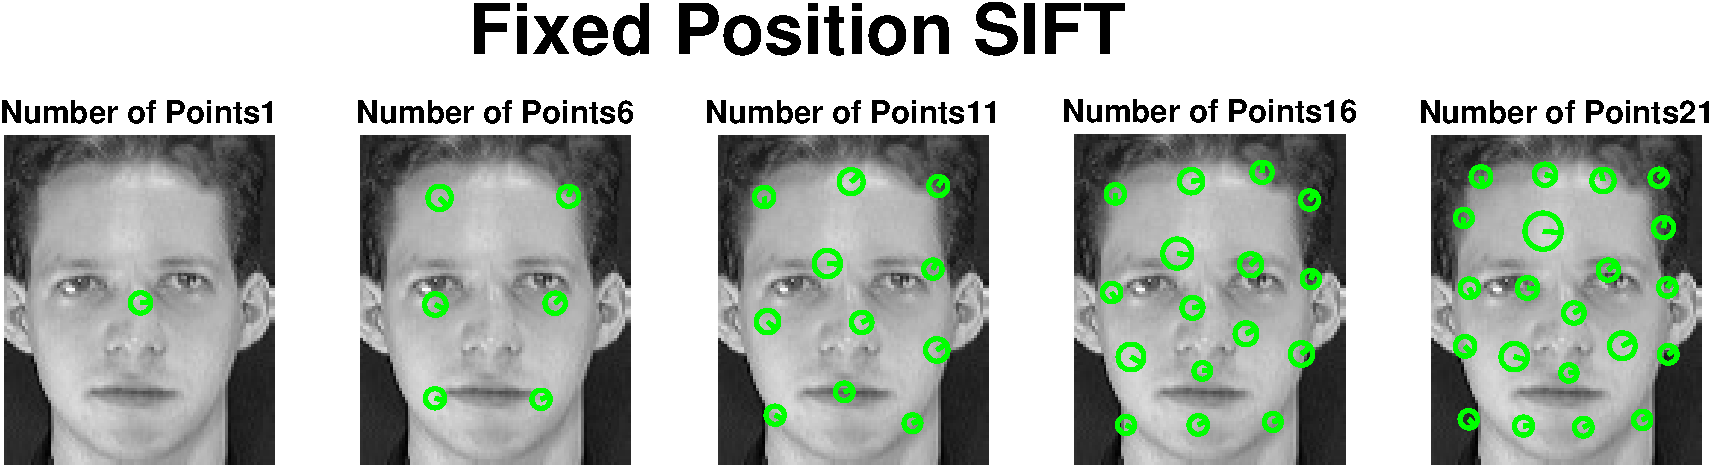
\includegraphics[width=\MyFactor\textwidth]{Img/c3/sift_fixedp} 
		\captionof{figure}{Kmeans计算出的特征位置}
		}
		\end{minipage}
		\medskip
		\end{center}
		
	第二步是在线在这些固定的特征点计算对应特征空间的描述,和之前方法的第4步一致.计算出的特征空间的描述的全集就可以作为输入图像的全局特征.


\subsection{NBNN分类法}
由于SIFT的特性,本项目在上一节固定编码的同时,也结合SIFT特性实现了NBNN(Naive-Baysian Nearest Neighbor)算法\cite{boiman2008defense}.NBNN算法不需要对SIFT进行特殊的编码,同时可以并行运算.它是基于距离的运算,主要思想是:
	\begin{enumerate}
		\item 通常的编码方法,如BoW丢失了很多有用的细节信息,只是注意到了描述空间中的高频成分,但是通常来说样本最具区分性的特征空间是其低频成分.并不适合以计算距离为主的KNN算法
		\item 通常的编码算法中,计算的是图像和图像之间的距离,这限制了算法的泛化能力.应该计算图像和类别之间的距离.
	\end{enumerate}
	它的主要过程是:
	\begin{enumerate}
		\item 对于样本图片,求得每类所有图片的所有描述
		\item 对于测试图片,求得该张图片的所有描述
		\item 在某个类别的所有描述的空间内,搜索测试图片的每个描述的最近特征点,并求得它们总共的距离.也即求得:
			\begin{equation}
				dis = \Sigma_{i=1}^n  || d_i - NN_C(d_i)^2||
			\end{equation}
			其中$NN_C(d_i)$是特征$d_i$在类别C内最近的特征点.
			
		\item 对所有的类别都求得该距离,距离最近的就是测试图片所属的类别.
	\end{enumerate}

其缺点是涉及了很多的求最近点的过程,在没有优化的Matlab代码中,使用了KD树结构也需要很多时间才能完成分类.这部分原因是因为Matlab是脚本语言,对处理多重循环的速度不够快导致的,但是,同样不可否认这其中确实存在了很多的寻最近点的KD树查询过程.

\paragraph{NKNN并行加速}
值得一提的是,由于NKNN算法过于缓慢,笔者使用了CPU并行运算.它具体的加速部分是加速了之前描述的步骤1和步骤3,步骤1是构架KD森林的过程,花费时间并不多.步骤3是遍历KD森林的过程,是程序主要耗时的地方.对于每个测试样本,它需要让这个样本逐一和ORL数据库中40个类构成的KD树逐一求得最小距离,使用了多核加速后,从以前的一次查询一个类加速到了一次查询两个类.\newline


无论如何,KBNN算法只是基于距离的计算,可以被并行加速,同时有很高的识别度.

\section{相关实验}
参见\ref{sec:comp_local}.

\chapter{Model Evaluation}
\label{chap:eval}


%%% ++++++++++++++++++++++++++++++++++++++++++++++++++++++++++++++++++++++++++++++++++



\appendix
%%%
%% >>> Nomenclatures
%%
\begin{nomenclature}

\section*{Roman Characters}
%\nomenclatureitem[\textbf{Unit}]{\textbf{Symbol}}{\textbf{Description}}
%\nomenclatureitem{\textrm{a}}{empirical stoichiometric coefficient}
%\nomenclatureitem[$m/s$]{\textrm{c}}{frozon sound speed}

\section*{Greek Characters}
%\nomenclatureitem{\textbf{Symbol}}{\textbf{Description}}
%\nomenclatureitem{$\alpha$}{velocity transmission factor}
%\nomenclatureitem{$\beta$}{temperature transmission factor}

\section*{Subscripts}
%\nomenclatureitem{\textbf{Symbol}}{\textbf{Description}}
%\nomenclatureitem{$CJ$}{Chapman-Jouguet state}
%\nomenclatureitem{$c$}{convection}

\section*{Operators}
%\nomenclatureitem{\textbf{Symbol}}{\textbf{Description}}
%\nomenclatureitem{$\triangledown$}{difference}
%\nomenclatureitem{$\nabla$}{gradient operator}

\section*{Abbreviations}
%\nomenclatureitem{\textbf{Acronym}}{\textbf{Description}}
%\nomenclatureitem{CJ}{Chapman-Jouguet}
%\nomenclatureitem{ZND}{Zel'dovich-von Neumann-Doering}

\end{nomenclature} % roman character...

\chapter{中国科学院大学学位论文撰写要求}
学位论文是研究生科研工作成果的集中体现,是评判学位申请者学术水平、授予其学位的主要依据,是科研领域重要的文献资料。根据《科学技术报告、学位论文和学术论文的编写格式》(GB/T 7713-1987)、《学位论文编写规则》(GB/T 7713.1-2006)和《文后参考文献著录规则》(GB7714—87)等国家有关标准,结合中国科学院大学(以下简称“国科大”)的实际情况,特制订本规定。

\section{学位论文的一般要求}

学位论文必须是一篇(或由一组论文组成的一篇)系统的、完整的学术论文。学位论文应是学位申请者本人在导师的指导下独立完成的研究成果,除论文中已经注明引用的内容外,不得抄袭和剽窃他人成果。对学位论文研究做出重要贡献的个人和集体,均应在文中以明确方式标明。学位论文的学术观点必须明确,且立论正确,推理严谨,数据可靠,层次分明,文字正确、语言通畅,表述清晰,图、表、公式、单位等符合规范要求。

\section{学位论文的水平要求}

硕士学位论文要选择在基础学科或应用学科中有价值的课题,对所研究的课题有新的见解,并能表明作者在本门学科上掌握了坚实的基础理论和系统的专门知识,具有从事科学研究工作或独立担负专门技术工作的能力。

博士学位论文要选择在国际上属于学科前沿的课题或对国家经济建设和社会发展有重要意义的课题,要突出论文在科学和专门技术上的创新性和先进性,并能表明作者在本门学科领域掌握了坚实宽广的基础理论和系统深入的专门知识,具有独立从事科学研究工作的能力。

\section{撰写学位论文的语言及文字}

除外国来华留学生及外语专业研究生外,研究生学位论文一般应采用国家正式公布实施的简化汉字撰写;应采用国家法定的计量单位。学位论文中采用的术语、符号、代号在全文中必须统一,并符合规范化的要求。

外国来华留学生可用中文或英文撰写学位论文,但须采用中文封面,且应有详细的中文摘要。外语专业的学位论文等应用所学专业相应的语言撰写,摘要应使用中文和所学专业相应的语言对照撰写。

为了便于国际合作与交流,学位论文亦可有英文或其它文字的副本。

\section{学位论文的主要组成部分}

学位论文一般由以下几个部分组成:中文封面、英文封面、致谢、中文摘要、英文摘要(Abstract)、目录、正文、参考文献、附录、作者简历及攻读学位期间发表的学术论文与研究成果。

\begin{enumerate}
  \item 学位论文题目应当简明扼要地概括和反映出论文的核心内容,一般不宜超过25个汉字(符),英文题目一般不应超过150个字母,必要时可加副标题。

  \item 论文摘要包括中文摘要和英文摘要(Abstract)两部分。论文摘要应概括地反映出本论文的主要内容,主要说明本论文的研究目的、内容、方法、成果和结论。要突出本论文的创造性成果或新见解,不宜使用公式、图表,不标注引用文献。英文摘要(Abstract)应与中文摘要内容相对应。摘要最后另起一行,注明本文的关键词(3-5个),关键词是为了文献标引工作从论文中选取出来,用以表示全文主题内容信息的单词或术语。

  \item 正文是学位论文的主体,包括引言(或绪论)、论文主体及结论等部分。
    \begin{itemize}
      \item 引言(或绪论)应包括选题的背景和意义,国内外相关研究成果述评,本论文所要解决的问题、所运用的主要理论和方法、基本思路和论文结构等。引言应独立成章,用足够的文字叙述,不与摘要雷同。

      \item 论文主体由于涉及不同的学科,在选题、研究方法、结果表达方式等有很大的差异,不作统一的规定。但必须严格遵循本学科国际通行的学术规范,言之成理,论据可靠,实事求是,合乎逻辑,层次分明,简练可读。

      \item 结论是对整个论文主要成果的总结,应明确、精炼、完整、准确。结论应明确指出本研究的创新点,对论文的学术价值和应用价值等加以预测和评价,说明研究中尚难解决的问题,并提出今后进一步在本研究方向进行研究工作的设想或建议。应严格区分本人研究成果与他人科研成果的界限。
    \end{itemize}

  \item 参考文献应本着严谨求实的科学态度,凡学位论文中有引用或参考、借用他人成果之处,均应按不同学科论文的引用规范,列于文末(通篇正文之后)。需正确区分直接引用和转引并明确加以标注。

  \item 学位论文印刷及装订要求:学位论文用A4标准纸打印、印刷或复印,按顺序装订成册。自中文摘要起双面印刷,之前部分单面印刷。论文必须用线装或热胶装订,不使用钉子装订。学位论文封面采用国科大统一规定的学位论文封面格式,封面用纸一般为150克(需保证论文封面印刷质量,字迹清晰、不脱落),博士学位论文封面颜色为红色,硕士学位论文封面颜色为蓝色。

  \item 学位论文的提交、保存与使用:学位申请者需按规定向国科大提交学位论文的印刷本和电子版,印刷本和电子版在内容与形式上应完全一致;国科大有权保存学位论文的印刷本和电子版,并提供目录检索与阅览服务,可以采用影印、缩印、数字化或其它复制手段保存学位论文;研究所、国科大有义务保护论文作者的知识产权。涉密学位论文在解密后,须按此规定执行。

  \item 本规定自印发之日起施行【2013年04月07日】,解释权属于校学位评定委员会,由国科大学位办公室负责解释。原《中国科学院研究生院研究生学位论文撰写规定》(院发学位字〔2012〕31号)同时废止。
\end{enumerate}


\backmatter

\bibliography{Biblio/Myrefs}
\bibliographystyle{unsrt}
\intotoc{参考文献}

%%%%
%%%% >>> Published papers
%%%
%\begin{publications}
%
%
%\end{publications}
%
%%%
%%%% >>> Resume if necessary
%%%
%\begin{resume}
%
%\paragraph{作者基本情况}
%
%\paragraph{联系方式}\mbox{}\\
%
%E-mail: 1275963@gmail.com
%
%\end{resume}
%
%%%
%%%% >>> Acknowledgements
%%%
%\begin{thanks}
%
%谨把本文献给我最敬爱的父亲!
%
%\end{thanks}
 % credits..
\end{document}

